\documentclass[12pt,a4paper]{article}
\usepackage[a4paper, margin=0.8in, headheight=14pt]{geometry}
\usepackage{fontspec}
\usepackage{unicode-math}
\setmainfont{TeX Gyre Pagella}
\setmonofont[Scale=0.88]{TeX Gyre Cursor}
\setmathfont{Latin Modern Math}
\usepackage{xcolor}
\usepackage{colortbl}
\usepackage{titlesec}
\usepackage{enumitem}
\usepackage{tabularx}
\usepackage{booktabs}
\usepackage{array}
\usepackage{amsmath}
\usepackage{tikz}
\usetikzlibrary{shapes.geometric, arrows.meta, positioning, calc, fit, decorations.pathreplacing, decorations.pathmorphing, patterns, backgrounds}
\usepackage[american]{circuitikz}
\usepackage{tcolorbox}
\tcbuselibrary{skins, breakable}
\usepackage{etoolbox}
\usepackage{hyperref}
\usepackage{fancyhdr}
\usepackage{graphicx}
\usepackage{microtype}
\hyphenpenalty=10000
\exhyphenpenalty=10000
\sloppy
\usepackage{caption}
\usepackage{setspace}
\usepackage{multirow}
\usepackage{tocloft}
\newcommand{\Q}[1]{\textbf{#1}\par\noindent\ignorespaces}
\definecolor{myred}{RGB}{196,30,58}
\definecolor{mydark}{RGB}{30,30,50}
\definecolor{mygreen}{RGB}{14,120,80}
\definecolor{myteal}{RGB}{0,130,140}
\definecolor{myamber}{RGB}{180,100,0}
\definecolor{mypurple}{RGB}{100,30,160}
\definecolor{mygray}{RGB}{246,247,249}
\definecolor{mgframe}{RGB}{180,185,200}
\definecolor{watermark}{RGB}{145,150,170}
\definecolor{hdrred}{RGB}{250,232,235}
\definecolor{hdrgreen}{RGB}{220,244,233}
\definecolor{hdrteal}{RGB}{220,242,244}
\definecolor{hdramber}{RGB}{253,242,215}
\definecolor{hdrpurple}{RGB}{238,228,255}
\definecolor{hdrgray}{RGB}{238,240,245}
\definecolor{rowalt}{RGB}{250,251,253}
\AfterEndEnvironment{tcolorbox}{\color{mydark}}

\titleformat{\section}{\large\bfseries\color{myred}}{\thesection.}{0.5em}{}[\vspace{1pt}{\color{myred}\rule{\linewidth}{0.8pt}}]
\titleformat{\subsection}{\normalsize\bfseries\color{myteal}}{\thesubsection}{0.5em}{}
\titlespacing*{\section}{0pt}{18pt}{7pt}
\titlespacing*{\subsection}{0pt}{11pt}{4pt}
\setlength{\parindent}{0pt}
\setlength{\parskip}{4pt}
\renewcommand{\cfttoctitlefont}{\large\bfseries\color{myred}}
\renewcommand{\cftaftertoctitle}{\par\noindent{\color{myred}\rule{\linewidth}{0.8pt}}}
\setlength{\cftbeforetoctitleskip}{0pt}
\setlength{\cftaftertoctitleskip}{6pt}
\renewcommand{\cftsecfont}{\normalsize\bfseries\color{mydark}}
\renewcommand{\cftsecpagefont}{\normalsize\bfseries\color{mydark}}
\renewcommand{\cftsecleader}{\cftdotfill{\cftdotsep}}
\setlength{\cftbeforesecskip}{7pt}
\renewcommand{\cftsubsecfont}{\small\color{mydark}}
\renewcommand{\cftsubsecpagefont}{\small\color{mydark}}
\setlength{\cftbeforesubsecskip}{3pt}
\setlength{\cftsubsecindent}{1.4em}
\renewcommand{\cftpartfont}{\normalsize\bfseries\color{myteal}}
\renewcommand{\cftpartpagefont}{\normalsize\bfseries\color{myteal}}
\setlength{\cftbeforepartskip}{14pt}
\renewcommand{\arraystretch}{1.45}
\setlength{\tabcolsep}{6pt}
\arrayrulecolor{mydark}
\newcolumntype{B}[1]{>{\small\bfseries\raggedright\arraybackslash}m{#1}}
\newcolumntype{C}[1]{>{\centering\arraybackslash}m{#1}}
\newcolumntype{Y}{>{\small\raggedright\arraybackslash}X}
\renewcommand{\tabularxcolumn}[1]{m{#1}}
\newcommand{\currmodule}{Module 1}
\pagestyle{fancy}
\fancyhf{}
\fancyhead[L]{\small\color{myred}\textbf{OE-EC803B}\;\color{mydark}--- Big Data Analysis}
\fancyhead[R]{\small\color{myteal}\textbf{\currmodule\ Notes}}
\fancyfoot[C]{\small\color{mydark}\thepage}
\fancyfoot[R]{\small\color{watermark}\textit{\copyright\ Biraj}}
\renewcommand{\headrulewidth}{0.5pt}
\renewcommand{\footrulewidth}{0.3pt}

\hypersetup{colorlinks=true, linkcolor=myteal, urlcolor=myteal,
  pdfauthor={Biraj Sarkar},
  pdftitle={OE-EC803B --- Combined Notes}}

\tcbset{
  tikzbox/.style={colback=mygray, colframe=mgframe, boxrule=0.6pt, arc=4pt,
    left=8pt, right=8pt, top=6pt, bottom=6pt,
    colbacktitle=mgframe, coltitle=mydark, fonttitle=\small\bfseries, unbreakable},
  defbox/.style={colback=hdrgreen, colframe=mygreen, boxrule=0.8pt, arc=4pt,
    left=9pt, right=9pt, top=6pt, bottom=6pt,
    colbacktitle=mygreen, coltitle=white, fonttitle=\small\bfseries},
  formulabox/.style={colback=hdrteal, colframe=myteal, boxrule=0.8pt, arc=4pt,
    left=9pt, right=9pt, top=7pt, bottom=7pt,
    colbacktitle=myteal, coltitle=white, fonttitle=\small\bfseries},
  examplebox/.style={colback=hdramber, colframe=myamber, boxrule=0.8pt, arc=4pt,
    left=9pt, right=9pt, top=6pt, bottom=6pt,
    colbacktitle=myamber, coltitle=white, fonttitle=\small\bfseries},
  masonbox/.style={colback=hdrpurple, colframe=mypurple, boxrule=0.8pt, arc=4pt,
    left=9pt, right=9pt, top=6pt, bottom=6pt,
    colbacktitle=mypurple, coltitle=white, fonttitle=\small\bfseries},
  exambox/.style={colback=hdrpurple, colframe=mypurple, boxrule=1pt, arc=5pt,
    left=10pt, right=10pt, top=8pt, bottom=8pt,
    colbacktitle=mypurple, coltitle=white, fonttitle=\bfseries,
    breakable, title after break={\textbf{Frequently Asked / Viva Questions (contd.)}}}
}
\tcbset{breakable}
\tcbset{coltext=mydark}
\tcbset{after={\color{mydark}}}

\tikzset{
  block/.style={rectangle, draw=myteal, fill=hdrteal,
    text width=2.2cm, align=center, minimum height=0.9cm,
    font=\small, rounded corners=3pt, line width=0.7pt},
  redblock/.style={rectangle, draw=myred, fill=hdrred,
    text width=2.2cm, align=center, minimum height=0.9cm,
    font=\small, rounded corners=3pt, line width=0.7pt},
  arrow/.style={-Stealth, thick, color=mydark},
  redarrow/.style={-Stealth, thick, color=myred},
  line/.style={thick, color=mydark}
}

\newcommand{\modulestart}[2]{%
  \clearpage
  \renewcommand{\currmodule}{Module #1}%
  \renewcommand{\theHsection}{mod#1.\arabic{section}}%
  \renewcommand{\theHsubsection}{\theHsection.\arabic{subsection}}%
  \renewcommand{\theHsubsubsection}{\theHsubsection.\arabic{subsubsection}}%
  \phantomsection
  \addcontentsline{toc}{part}{Module #1: #2}%
  \setcounter{section}{0}%
  \begin{center}
    \vspace*{1.0cm}
    {\Huge\bfseries\color{myred} Module #1}\\[10pt]
    {\Large\bfseries\color{mydark} #2}\\[10pt]
    {\color{myred}\rule{0.55\linewidth}{1.2pt}}
  \end{center}
  \vspace{14pt}
}
\begin{document}

\thispagestyle{empty}

% ─── Page Border (TikZ Overlay) ────────────────────────────────────────────────
\begin{tikzpicture}[remember picture, overlay]
  % Outer border (fine line in mgframe)
  \draw[color=mgframe, line width=1.5pt] 
    ($(current page.north west) + (0.6in, -0.6in)$) rectangle 
    ($(current page.south east) + (-0.6in, 0.6in)$);
  % Inner border (finer accent line in myred)
  \draw[color=myred, line width=0.8pt] 
    ($(current page.north west) + (0.65in, -0.65in)$) rectangle 
    ($(current page.south east) + (-0.65in, 0.65in)$);
\end{tikzpicture}

\vspace*{1.0cm}
\begin{center}
  {\Huge\bfseries\color{myred} OE-EC803B}\\[10pt]
  {\LARGE\bfseries\color{mydark} Big Data Analysis}\\[20pt]
  {\color{myred}\rule{0.7\linewidth}{1.5pt}}\\[18pt]
  {\Large\color{myteal}\textbf{Combined Module Notes}}\\[8pt]
  {\large\color{mydark} Modules 1 -- 6}\\[40pt]
  {\normalsize\color{mydark} Semester VIII \quad$\bullet$\quad ECE \quad$\bullet$\quad 3 Credits}\\[12pt]
  {\normalsize\color{mydark} CGEC \;$|$\; B.Tech ECE (2023--27)}
\end{center}
\vspace{1.0cm}
\begin{center}
  \begin{tcolorbox}[colback=mygray, colframe=mgframe, boxrule=0.5pt, arc=3pt, width=0.85\linewidth]
    \centering\small\color{mydark}
    \textbf{Disclaimer / Study Guide Notice:}\\
    These are condensed \textbf{Short Notes} focusing on core theory, key formulas, block/circuit diagrams, and standard viva Q\&As for university exam revision. Exhaustive numerical practice problems and derivation edge cases are not covered. This serves as a quick-revision reference guide for students.
  \end{tcolorbox}
\end{center}
\vfill
\vspace{0.6cm}
\begin{center}
  {\large\bfseries\color{mypurple} Biraj Sarkar}\\[16pt]
  {\footnotesize\color{watermark}\textbf{IN ASSOCIATION WITH}}\\[8pt]
  {\small\bfseries\color{mydark} MAKAUT Wingman \quad$\bullet$\quad MAKAUT Future Minds}\\[12pt]
  {\large\bfseries\color{myteal} Cooch Behar Government Engineering College}
\end{center}
\vfill
\begin{center}{\small\color{watermark}\textit{Exam-Ready Notes}}\end{center}
\clearpage

\hypersetup{linkcolor=mydark}
\tableofcontents
\hypersetup{linkcolor=myteal}
\clearpage

% -- Module 0 -----------------------------------------------------------------
\modulestart{0}{Java Programming \& OOP Foundations}

\section{Java Programming \& OOP Foundations}
% ===============================================================================

Distributed frameworks in the Hadoop Ecosystem are heavily built on Java. A strong grasp of Java's runtime environment and Object-Oriented Programming (OOP) paradigms is essential to understand HDFS mechanics and MapReduce workflows.

\begin{tcolorbox}[defbox, title={Java Virtual Machine (JVM)}]
  The \textbf{Java Virtual Machine (JVM)} is an abstract computing machine that provides a runtime environment in which Java bytecode can be executed. It acts as an engine that drives the execution of Java code, converting bytecode to machine-specific instructions and managing system memory.
\end{tcolorbox}

\subsection{Object-Oriented Programming (OOP) Principles}
Java uses four primary OOP pillars which map directly to distributed programming:
\begin{itemize}[leftmargin=*, itemsep=3pt]
  \item \textbf{Encapsulation:} Bundling fields and methods within a single class and restricting direct access (using access modifiers like `private`, `protected`, `public`) to protect the internal state of objects.
  \item \textbf{Inheritance:} Allowing a class (subclass) to inherit fields and methods from another class (superclass). In Hadoop, custom mappers and reducers inherit from base API classes.
  \item \textbf{Polymorphism:} The ability of an object to take on many forms. Used in Hadoop when custom serialized types implement interface contracts (e.g., overriding the `write()` and `readFields()` methods of the `Writable` interface).
  \item \textbf{Abstraction:} Hiding implementation details and showing only functional interfaces using `abstract` classes and `interfaces`.
\end{itemize}

\subsection{Java Collections Framework}
In MapReduce, intermediate values are held in collection data structures. The framework provides three primary categories of collections:

\par\vspace{6pt}\noindent
{\renewcommand{\arraystretch}{1.4}%
\begin{tabularx}{\linewidth}{|B{3.0cm}|Y|B{3.2cm}|Y|}
\hline
\textbf{Collection} & \textbf{Key Characteristics} & \textbf{Underlying Structure} & \textbf{Hadoop Use Case} \\
\hline
`ArrayList` & Ordered, indexable list. Allows duplicates. Resizes dynamically. & Resizable Array & Gathering list of values associated with a single key in Reducer. \\
\hline
`HashSet` & Unordered collection. No duplicates allowed. & Hash Table & Filtering out duplicate records or keys during processing. \\
\hline
`HashMap` & Key-value pairs storage. Unique keys. Fast search. & Hash Table + Linked List & Local in-memory caching and Map-Side Joins. \\
\hline
\end{tabularx}}

\subsection{JVM Memory Management}
The JVM splits its runtime memory into distinct regions. Understanding this is key to debugging Out-Of-Memory (OOM) errors in Hadoop:
\begin{itemize}[leftmargin=*, itemsep=3pt]
  \item \textbf{Stack Memory:} Stores local variables and method execution frames. Allocation and deallocation are managed automatically.
  \item \textbf{Heap Memory:} Stores all objects instantiated via the `new` keyword. Managed by the JVM \textbf{Garbage Collector (GC)}. If MapReduce buffers grow too large, Heap memory exhaustion triggers a JVM crash.
\end{itemize}

\begin{tcolorbox}[tikzbox, title={JVM Heap and Stack Memory Structure}]
\centering
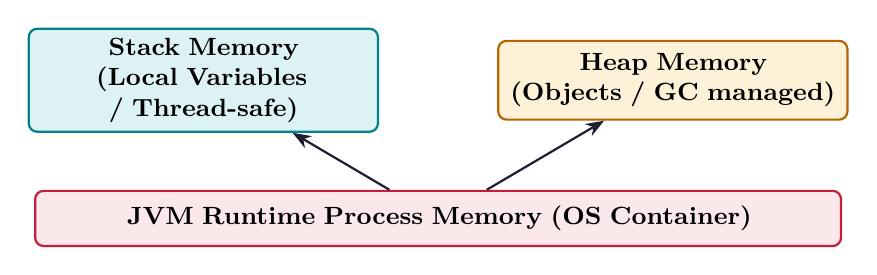
\begin{tikzpicture}[node distance=1.2cm and 1.5cm,
  mblock/.style={rectangle, draw=myteal, fill=hdrteal, text width=4.2cm, align=center, minimum height=1.0cm, font=\small\bfseries, rounded corners=3pt, line width=0.8pt},
  gblock/.style={rectangle, draw=myamber, fill=hdramber, text width=4.2cm, align=center, minimum height=1.0cm, font=\small\bfseries, rounded corners=3pt, line width=0.8pt},
  rblock/.style={rectangle, draw=myred, fill=hdrred, text width=10.0cm, align=center, minimum height=0.7cm, font=\small\bfseries, rounded corners=3pt, line width=0.8pt}]

  % Stack Nodes
  \node[mblock] (stack) {Stack Memory\\(Local Variables / Thread-safe)};
  
  % Heap Nodes
  \node[gblock, right=of stack] (heap) {Heap Memory\\(Objects / GC managed)};

  % Shared System Node
  \node[rblock, below=0.8cm of $(stack.south)!0.5!(heap.south)$] (jvm) {JVM Runtime Process Memory (OS Container)};

  % Connections
  \draw[arrow] (jvm) -- (stack);
  \draw[arrow] (jvm) -- (heap);
  
\end{tikzpicture}
\end{tcolorbox}

% ===============================================================================
\section{Structured Query Language (SQL) \& Relational Algebra}
% ===============================================================================

Data warehouse systems like Apache Hive use HiveQL, which is a dialect of SQL. Distributed querying translates SQL declarations into computational graphs.

\begin{tcolorbox}[defbox, title={Relational Databases vs. Hadoop Queries}]
  Traditional databases use \textbf{Schema-on-Write}, validating data constraints during insertion. SQL engines on Hadoop (like Hive and Big SQL) use \textbf{Schema-on-Read}, overlaying structure on top of raw file streams (e.g., text, CSV, ORC) at query execution time.
\end{tcolorbox}

\subsection{Logical Execution Order of an SQL Query}
While SQL queries are written starting with the `SELECT` clause, the SQL compiler executes operations in a different logical sequence:

\begin{tcolorbox}[formulabox, title={Logical SQL Execution Order}]
  $$\text{FROM} \longrightarrow \text{JOIN} \longrightarrow \text{WHERE} \longrightarrow \text{GROUP BY} \longrightarrow \text{HAVING} \longrightarrow \text{SELECT} \longrightarrow \text{ORDER BY}$$
  \begin{itemize}[leftmargin=*, noitemsep]
    \item \textbf{FROM/JOIN:} Identifies target datasets and links them.
    \item \textbf{WHERE:} Filters rows based on non-aggregated predicates.
    \item \textbf{GROUP BY:} Groups rows based on key values.
    \item \textbf{HAVING:} Filters groups using aggregate functions (e.g., `HAVING count(*) > 5`).
    \item \textbf{SELECT:} Projects fields and calculates functions.
    \item \textbf{ORDER BY:} Sorts output (very expensive in distributed systems as it forces global sorting).
  \end{itemize}
\end{tcolorbox}

\subsection{SQL Joins}
Joins are fundamental operations that merge datasets horizontally on a matching key column:
\begin{itemize}[leftmargin=*, itemsep=3pt]
  \item \textbf{Inner Join:} Returns records that have matching values in both tables.
  \item \textbf{Left (Outer) Join:} Returns all records from the left table, and matched records from the right table. Fill with `NULL` on the right side if no match.
  \item \textbf{Right (Outer) Join:} Returns all records from the right table, and matched records from the left table.
  \item \textbf{Full (Outer) Join:} Returns all records when there is a match in either left or right table.
\end{itemize}

\begin{tcolorbox}[tikzbox, title={SQL Joins Visual Representation}]
\centering
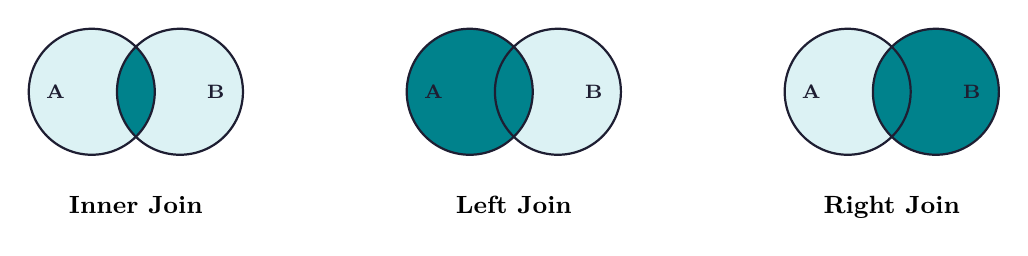
\begin{tikzpicture}[scale=0.8]
  % Set styles
  \tikzset{set/.style={circle, minimum size=2.8cm, fill opacity=0.4, line width=0.8pt}}

  % Inner Join Group
  \begin{scope}[shift={(0,0)}]
    \fill[hdrteal] (0,0) circle (1.0cm);
    \fill[hdrteal] (1.4,0) circle (1.0cm);
    \begin{scope}
      \clip (0,0) circle (1.0cm);
      \fill[myteal] (1.4,0) circle (1.0cm);
    \end{scope}
    \draw[line] (0,0) circle (1.0cm) node[left=6pt, font=\scriptsize\bfseries] {A};
    \draw[line] (1.4,0) circle (1.0cm) node[right=6pt, font=\scriptsize\bfseries] {B};
    \node[below=1.2cm] at (0.7,0) {\small\bfseries Inner Join};
  \end{scope}

  % Left Join Group
  \begin{scope}[shift={(6.0,0)}]
    \fill[hdrteal] (1.4,0) circle (1.0cm);
    \fill[myteal] (0,0) circle (1.0cm);
    \draw[line] (0,0) circle (1.0cm) node[left=6pt, font=\scriptsize\bfseries] {A};
    \draw[line] (1.4,0) circle (1.0cm) node[right=6pt, font=\scriptsize\bfseries] {B};
    \node[below=1.2cm] at (0.7,0) {\small\bfseries Left Join};
  \end{scope}

  % Right Join Group
  \begin{scope}[shift={(12.0,0)}]
    \fill[hdrteal] (0,0) circle (1.0cm);
    \fill[myteal] (1.4,0) circle (1.0cm);
    \draw[line] (0,0) circle (1.0cm) node[left=6pt, font=\scriptsize\bfseries] {A};
    \draw[line] (1.4,0) circle (1.0cm) node[right=6pt, font=\scriptsize\bfseries] {B};
    \node[below=1.2cm] at (0.7,0) {\small\bfseries Right Join};
  \end{scope}
\end{tikzpicture}
\end{tcolorbox}

\subsection{Subqueries and Common Table Expressions (CTEs)}
\begin{itemize}[leftmargin=*, itemsep=3pt]
  \item \textbf{Subquery:} A query nested inside another SQL statement. It can return scalar values, single columns, or tables (e.g., `SELECT * FROM emp WHERE salary > (SELECT AVG(salary) FROM emp)`).
  \item \textbf{Common Table Expression (CTE):} A temporary named result set defined using the `WITH` keyword, which improves readability compared to nested subqueries:
\end{itemize}

\begin{tcolorbox}[examplebox, title={Common Table Expression (CTE) Syntax}]
  \begin{spacing}{0.95}
  \begin{verbatim}
  WITH DeptAvgSalary AS (
      SELECT dept_id, AVG(salary) AS avg_sal
      FROM employees
      GROUP BY dept_id
  )
  SELECT e.name, e.salary, d.avg_sal
  FROM employees e
  JOIN DeptAvgSalary d ON e.dept_id = d.dept_id;
  \end{verbatim}
  \end{spacing}
\end{tcolorbox}

% ===============================================================================
\section{Linux Command Line \& Unix Text Processing}
% ===============================================================================

Hadoop CLI commands mimic standard Linux file system operations. Exposure to Unix text processing tools is essential for filtering, parsing, and verifying datasets before importing them.

\begin{tcolorbox}[defbox, title={Unix Streams}]
  Unix systems model communications via three standard input/output channels (streams):
  \begin{itemize}[leftmargin=*, noitemsep]
    \item \textbf{stdin (0):} Standard Input stream (default: keyboard).
    \item \textbf{stdout (1):} Standard Output stream (default: terminal screen).
    \item \textbf{stderr (2):} Standard Error stream (default: terminal screen).
  \end{itemize}
\end{tcolorbox}

\subsection{Core File Manipulation Commands}
\begin{itemize}[leftmargin=*, itemsep=3pt]
  \item `cd <dir>`: Change current working directory.
  \item `ls -la`: List directory contents showing file size, permissions, and hidden files.
  \item `mkdir -p <path>`: Create directories recursively without throwing errors if they exist.
  \item `cp -r <src> <dest>`: Copy files and directories recursively.
  \item `mv <src> <dest>`: Move or rename files.
  \item `rm -rf <path>`: Recursively force delete files or directories.
  \item `chmod 755 <file>`: Modify file read-write-execute permissions (rwxr-xr-x).
\end{itemize}

\subsection{Redirections and Pipelines}
Commands can output data to files or other commands instead of printing to the terminal:
\begin{itemize}[leftmargin=*, itemsep=3pt]
  \item \textbf{Redirections:} Redirect outputs or inputs to files.
        \begin{itemize}[leftmargin=*, noitemsep]
          \item `>`: Redirects `stdout` to a file (overwriting existing content).
          \item `>>`: Appends `stdout` to a file.
          \item `2>`: Redirects `stderr` to a file.
        \end{itemize}
  \item \textbf{Pipes (`|`):} Passes the `stdout` of one command as the `stdin` of the next command.
\end{itemize}

\begin{tcolorbox}[tikzbox, title={Pipeline Data Flow}]
\centering
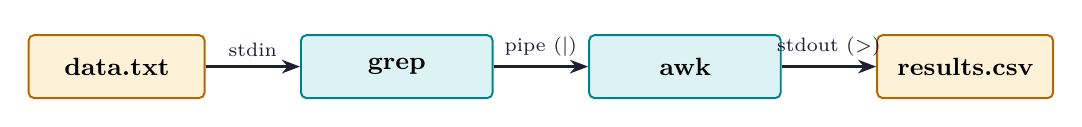
\begin{tikzpicture}[node distance=1.1cm and 1.2cm,
  cblock/.style={rectangle, draw=myteal, fill=hdrteal, text width=2.2cm, align=center, minimum height=0.8cm, font=\small\bfseries, rounded corners=2pt, line width=0.7pt},
  fblock/.style={rectangle, draw=myamber, fill=hdramber, text width=2.0cm, align=center, minimum height=0.8cm, font=\small\bfseries, rounded corners=2pt, line width=0.7pt}]

  % Nodes
  \node[fblock] (file) {data.txt};
  \node[cblock, right=of file] (c1) {grep};
  \node[cblock, right=of c1] (c2) {awk};
  \node[fblock, right=of c2] (out) {results.csv};

  % Paths
  \draw[arrow] (file) -- node[above, font=\scriptsize] {stdin} (c1);
  \draw[arrow] (c1) -- node[above, font=\scriptsize] {pipe (|)} (c2);
  \draw[arrow] (c2) -- node[above, font=\scriptsize] {stdout (>)} (out);

\end{tikzpicture}
\end{tcolorbox}

\subsection{Unix Text Processing Tools}
Hadoop Streaming allows using Unix programs as mappers and reducers. The core tools are:
\begin{itemize}[leftmargin=*, itemsep=3pt]
  \item `cat`: Concatenates and displays file contents.
  \item `grep <pattern>`: Searches for regular expression pattern matches within files.
  \item \texttt{awk}: A pattern scanning and processing language. Heavily used to extract columns (e.g., \texttt{awk '\{print \$2\}'} extracts the second space-separated field).
  \item `sed`: A stream editor for parsing and transforming text (e.g., substitute strings).
  \item `sort`: Sorts lines of text files alphabetically or numerically.
  \item `uniq`: Discards duplicate adjacent lines. Needs data to be pre-sorted.
\end{itemize}

\begin{tcolorbox}[examplebox, title={Common UNIX Text Processing Pipeline}]
  To find the top 5 most frequent error types from a log file:
  \begin{spacing}{0.95}
  \begin{verbatim}
  cat server.log | grep "ERROR" | awk '{print $5}' | sort | uniq -c | sort -nr | head -n 5
  \end{verbatim}
  \end{spacing}
  \textbf{Explanation:} 
  Step 1: Print file $\longrightarrow$ Step 2: Filter lines containing "ERROR" $\longrightarrow$ Step 3: Extract the fifth column $\longrightarrow$ Step 4: Sort columns $\longrightarrow$ Step 5: Count occurrences of unique elements $\longrightarrow$ Step 6: Sort counts numerically in descending order $\longrightarrow$ Step 7: Print top 5 lines.
\end{tcolorbox}

\newpage

% ═══════════════════════════════════════════════════════════════════════════════
% QUICK REVISION PAGE
% ═══════════════════════════════════════════════════════════════════════════════
\begin{center}
  {\large\bfseries\color{myred} Quick Revision --- Module 0}\\[3pt]
  {\small\color{mydark} Java Collections, SQL Queries \& Unix Pipelines $|$ OE-EC803B}
\end{center}
\noindent{\color{myred}\rule{\linewidth}{1.2pt}}
\vspace{8pt}

\begin{tcolorbox}[defbox, title={\textbf{One-Line Definitions}}]
\begin{itemize}[leftmargin=*, itemsep=3pt, topsep=0pt]
  \item \textbf{Polymorphism:} The OOP capability to invoke object-specific methods via interface abstractions.
  \item \textbf{Schema-on-Read:} A data schema validation approach where structure is applied only when reading files.
  \item \textbf{Common Table Expression (CTE):} A temporary named result set defined locally within an SQL query block.
  \item \textbf{Unix Pipe:} A mechanism that directs the standard output of one command to the standard input of another.
  \item \textbf{Garbage Collector (GC):} A background JVM process that automatically reclaims memory by deleting unreferenced objects.
\end{itemize}
\end{tcolorbox}

\vspace{6pt}

\begin{tcolorbox}[exambox, title={\textbf{Frequently Asked / Viva Questions}}]
\begin{enumerate}[leftmargin=*, topsep=0pt, label=\textbf{Q\arabic*.}, itemsep=5pt]
  \item \Q{Why is Java memory management critical in Hadoop MapReduce jobs?}
        Custom mapper and reducer code instantiates objects inside JVM heap containers. If collections (like lists or hash maps) grow indefinitely without boundary checks, JVM Heap runs out of memory, leading to job failure.
        
  \item \Q{Compare SQL's WHERE and HAVING clauses.}
        The `WHERE` clause filters individual rows before grouping operations occur. The `HAVING` clause filters aggregated groups after the `GROUP BY` clause has been processed.
        
  \item \Q{Explain the utility of SQL Subqueries vs. CTEs.}
        Subqueries are nested expressions that can make queries complex and hard to read. Common Table Expressions (CTEs) define clear, modular virtual tables using `WITH`, facilitating compiler optimization and improving readability.
        
  \item \Q{What does the command ``chmod 755 script.sh'' accomplish?}
        It sets file permissions: Owner receives full permissions (Read=4, Write=2, Execute=1 $\to$ 7). Group and Others receive Read and Execute permissions (Read=4, Execute=1 $\to$ 5).
        
  \item \Q{Why must ``uniq'' be preceded by a ``sort'' command in Unix pipelines?}
        The `uniq` command only matches and filters out adjacent duplicate lines. If duplicate records are scattered, `uniq` will miss them. Pre-sorting groups duplicate lines together.
        
  \item \Q{What is the difference between ``>'' and ``>>'' in Unix Shell?}
        `>` redirects standard output to a file, overwriting the file's current contents. `>>` redirects output to a file, appending the output at the end of the file.
        
  \item \Q{Describe the JVM Stack vs. Heap memory allocations.}
        Stack allocation is temporary, storing thread execution states and primitive local variables. Heap stores dynamic class objects that require garbage collection.
        
  \item \Q{What is the time complexity of looking up a key in a HashMap?}
        On average, `HashMap` lookup has $O(1)$ constant time complexity. In the worst case (with hash collisions), it defaults to $O(n)$ or $O(\log n)$.
        
  \item \Q{Explain standard error (stderr) redirection in shell.}
        Errors bypass standard output redirection. To capture error logs, redirect standard error using `2>` (e.g., `command > out.txt 2> error.log`).
        
  \item \Q{What is the difference between Schema-on-Write and Schema-on-Read?}
        Schema-on-Write enforces schema definitions when writing data to relational tables, rejecting formatting violations. Schema-on-Read stores raw data files as-is, parsing formatting layouts dynamically during queries.
\end{enumerate}
\end{tcolorbox}

\vspace{6pt}

\begin{tcolorbox}[tikzbox, title={\textbf{Comparison Snapshot}}]
\textbf{Foundational Paradigm Comparisons:}\par\vspace{6pt}\noindent
{\renewcommand{\arraystretch}{1.4}%
\begin{tabularx}{\linewidth}{|B{3.2cm}|Y|Y|}
\hline
\textbf{Feature} & \textbf{SQL Database Engine} & \textbf{Unix Command Line} \\
\hline
Execution Paradigm & Declarative (describe \textit{what} data to fetch) & Procedural (pipe \textit{how} data flows through tools) \\
\hline
Primary Objective & Structured relational database querying & General-purpose file processing and system control \\
\hline
Data Structures & Tables, columns, index structures & Text streams, byte buffers, files \\
\hline
Scaling Pattern & Relies on query planners and indexes & Relies on stream processing buffers \\
\hline
Optimization & Handled by query optimizer engines & Handled manually by pipeline construction \\
\hline
\end{tabularx}}
\end{tcolorbox}


% -- Module 1 -----------------------------------------------------------------
\modulestart{1}{Types of Digital Data}

\section{Types of Digital Data}
% ===============================================================================

Digital data represents any information stored, processed, or transmitted electronically. In modern computer systems, digital data is classified into three categories based on its structural characteristics:

\begin{tcolorbox}[defbox, title={Classification of Digital Data}]
  \textbf{Digital Data} is categorized into three types:
  \begin{enumerate}[leftmargin=*, noitemsep]
    \item \textbf{Structured Data:} Highly organized data conforming to a rigid pre-defined schema (e.g., relational databases).
    \item \textbf{Semi-Structured Data:} Data containing internal identifiers, tags, or markers (no rigid schema, but self-describing; e.g., JSON, XML).
    \item \textbf{Unstructured Data:} Data lacking any predefined structure or model (e.g., videos, PDF documents, raw text).
  \end{enumerate}
\end{tcolorbox}

\subsection{Detailed Characteristics}
\begin{itemize}[leftmargin=*, itemsep=4pt]
  \item \textbf{Structured Data:}
    Stored in tables with rows and columns. Uses Structured Query Language (SQL) for retrieval. It has fixed fields and schemas.
    \textit{Examples:} Relational Databases (RDBMS), CSV files, spreadsheets.
  \item \textbf{Semi-Structured Data:}
    Does not conform to the formal structure of databases but contains tags or markers to separate data elements and enforce hierarchies.
    \textit{Examples:} XML documents, JSON strings, HTML files, NoSQL Key-Value records.
  \item \textbf{Unstructured Data:}
    Represents the majority of real-world data (estimated at 80--90\% of all enterprise data). It is difficult to store in standard tabular formats.
    \textit{Examples:} MP3 files, MP4 videos, JPEG images, raw logs, emails, PDF manuals.
  \end{itemize}

\par\vspace{6pt}\noindent
{\renewcommand{\arraystretch}{1.4}%
\begin{tabularx}{\linewidth}{|B{2.8cm}|Y|Y|Y|}
\hline
\textbf{Parameter} & \textbf{Structured Data} & \textbf{Semi-Structured Data} & \textbf{Unstructured Data} \\
\hline
Format & Tabular (Rows/Columns) & Tags/Key-value pairs & No specific structure \\
\hline
Schema & Schema-on-write (rigid) & Schema-on-read (flexible) & No schema applied \\
\hline
Storage & RDBMS (SQL Server, MySQL) & NoSQL databases, XML files & NoSQL databases, Data Lakes \\
\hline
Flexibility & Very low & Moderate & High \\
\hline
Scale & Hard to scale horizontally & Scalable horizontally & Highly scalable \\
\hline
Querying & Structured SQL queries & XQuery, JSON Path & Search indices, NLP, ML \\
\hline
\end{tabularx}}

% ===============================================================================
\section{Introduction to Big Data}
% ===============================================================================

\begin{tcolorbox}[defbox, title={Big Data}]
  \textbf{Big Data} refers to datasets whose size (volume), complexity (variety), and rate of growth (velocity) are so large that traditional data processing application software (such as relational database management systems) are inadequate to capture, store, manage, and process them within a tolerable elapsed time.
\end{tcolorbox}

\subsection{The 5Vs of Big Data}
The core dimensions defining Big Data are historically known as the \textbf{3Vs} (Volume, Velocity, Variety), which have been expanded to the \textbf{5Vs} to reflect reliability and business value:

\begin{enumerate}[leftmargin=*, itemsep=3pt]
  \item \textbf{Volume:} The sheer scale of data generated. Measured in Terabytes (TB), Petabytes (PB), or Exabytes (EB).
  \item \textbf{Velocity:} The speed at which new data is generated, transmitted, and processed in real-time (e.g., social media feeds, sensor streams).
  \item \textbf{Variety:} The structural diversity of data types (structured, semi-structured, and unstructured data coming from various sources).
  \item \textbf{Veracity:} The trustworthiness, quality, and accuracy of the incoming data (noise reduction, handling missing values).
  \item \textbf{Value:} The actionable business insights extracted from the data, turning raw bits into commercial or operational intelligence.
\end{enumerate}

\begin{tcolorbox}[tikzbox, title={The 5Vs of Big Data}]
\centering
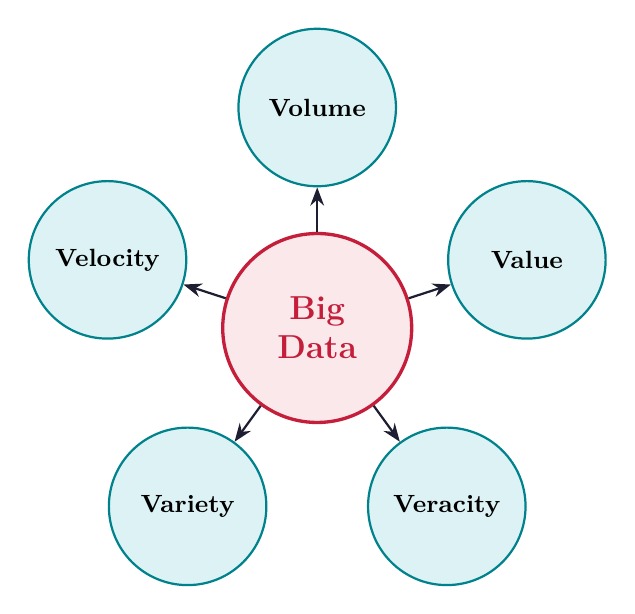
\begin{tikzpicture}[node distance=1.2cm,
  vnode/.style={circle, draw=myteal, fill=hdrteal, minimum size=2.0cm, align=center, font=\small\bfseries, line width=0.8pt},
  centerbox/.style={circle, draw=myred, fill=hdrred, minimum size=2.4cm, align=center, font=\large\bfseries\color{myred}, line width=1.2pt},
  carrow/.style={-Stealth, thick, color=mydark}]

  % Center node
  \node[centerbox] (bd) at (0,0) {Big\\Data};

  % Satellite nodes
  \node[vnode] (vol) at (90:2.8cm) {Volume};
  \node[vnode] (vel) at (162:2.8cm) {Velocity};
  \node[vnode] (var) at (234:2.8cm) {Variety};
  \node[vnode] (ver) at (306:2.8cm) {Veracity};
  \node[vnode] (val) at (18:2.8cm) {Value};

  % Connections
  \draw[carrow] (bd) -- (vol);
  \draw[carrow] (bd) -- (vel);
  \draw[carrow] (bd) -- (var);
  \draw[carrow] (bd) -- (ver);
  \draw[carrow] (bd) -- (val);

\end{tikzpicture}
\end{tcolorbox}

\subsection{Challenges of Traditional Database Systems (RDBMS)}
Traditional RDBMS architectures fail to handle Big Data due to several fundamental limits:
\begin{itemize}[leftmargin=*, itemsep=3pt]
  \item \textbf{Vertical Scaling (Scale-up) limits:} RDBMS scale by adding CPU, RAM, or storage to a single server. This has physical and cost limits. Big Data requires horizontal scaling (scaling out by adding cheap commodity nodes).
  \item \textbf{Rigid Schema Requirements:} RDBMS requires schema definitions before writing data. This prevents storing unstructured data or dynamic fields.
  \item \textbf{ACID Properties Overhead:} Locking rows/tables to maintain strict Consistency and Isolation creates severe latency spikes at high transaction speeds.
\end{itemize}

% ===============================================================================
\section{Big Data Analytics}
% ===============================================================================

\begin{tcolorbox}[defbox, title={Big Data Analytics}]
  \textbf{Big Data Analytics} is the process of examining large and varied datasets to uncover hidden patterns, unknown correlations, market trends, customer preferences, and other useful information to make informed business decisions.
\end{tcolorbox}

\subsection{Types of Big Data Analytics}
Analytics tasks are classified into four distinct stages based on complexity and value:

\begin{enumerate}[leftmargin=*, itemsep=3pt]
  \item \textbf{Descriptive Analytics (What happened?):} Summarizes historical data to identify trends and patterns (e.g., standard reports, dashboards).
  \item \textbf{Diagnostic Analytics (Why did it happen?):} Drill-down queries to identify the root cause of historical trends (e.g., analyzing customer churn).
  \item \textbf{Predictive Analytics (What is likely to happen?):} Uses statistical models, forecasting algorithms, and machine learning to estimate future outcomes.
  \item \textbf{Prescriptive Analytics (What should we do?):} Recommends action pathways based on simulations and optimization algorithms to capitalize on predictions.
\end{enumerate}

% ===============================================================================
\section{History and Architecture of Apache Hadoop}
% ===============================================================================

\subsection{History of Hadoop}
Hadoop was created by Doug Cutting and Mike Cafarella in 2005. It originated from work on Nutch, an open-source web crawler project.
\begin{itemize}[leftmargin=*, itemsep=3pt]
  \item It was inspired by Google's white papers on GFS (Google File System) published in 2003 and MapReduce framework published in 2004.
  \item Doug Cutting joined Yahoo! in 2006, and Yahoo! spun off Hadoop as an independent open-source project. In 2008, Apache Hadoop became a top-level project.
  \item Named after Doug Cutting's son's toy yellow elephant.
\end{itemize}

\subsection{Core Components of Apache Hadoop}
Hadoop provides a distributed software framework designed to run on clusters of commodity hardware.

\begin{tcolorbox}[formulabox, title={Core Hadoop Modules}]
  Hadoop's primary runtime architecture contains three core modules:
  \begin{enumerate}[leftmargin=*, noitemsep]
    \item \textbf{HDFS (Hadoop Distributed File System):} The distributed storage layer that splits files into blocks and distributes them across cluster nodes.
    \item \textbf{MapReduce:} The software programming framework for writing applications that process massive amounts of structured and unstructured data in parallel.
    \item \textbf{YARN (Yet Another Resource Negotiator):} The cluster resource management layer that schedules jobs and allocates CPU/RAM resources across the cluster.
  \end{enumerate}
\end{tcolorbox}

\subsection{Unix Tools vs. Hadoop}
Small datasets are processed locally using Unix utilities, whereas large datasets require distributed execution on Hadoop.

\par\vspace{6pt}\noindent
{\renewcommand{\arraystretch}{1.4}%
\begin{tabularx}{\linewidth}{|B{3.2cm}|Y|Y|}
\hline
\textbf{Parameter} & \textbf{Unix Utilities (grep, awk, sed)} & \textbf{Apache Hadoop} \\
\hline
Execution Location & Single local machine & Distributed cluster (scale-out) \\
\hline
Data Volume Limit & Limited by local RAM and disk size & Petabytes (scales linearly with nodes) \\
\hline
Processing Paradigm & Sequential processing (single-threaded pipes) & Parallel, distributed execution (MapReduce) \\
\hline
Fault Tolerance & None (if the shell script crashes, run aborts) & High (data blocks replicated; jobs rerun automatically) \\
\hline
Data Locality & Reads data to CPU over system bus & Pushes computation code directly to storage nodes \\
\hline
\end{tabularx}}

% ===============================================================================
\section{Hadoop Streaming}
% ===============================================================================

\begin{tcolorbox}[defbox, title={Hadoop Streaming}]
  \textbf{Hadoop Streaming} is a utility that comes bundled with the Hadoop distribution that allows users to create and run MapReduce jobs with any executable or script as the mapper and/or the reducer (e.g., Python, Perl, Bash) by exchanging data via standard input (`stdin`) and standard output (`stdout`).
\end{tcolorbox}

\subsection{Mechanism and Data Flow}
\begin{enumerate}[leftmargin=*, itemsep=3pt]
  \item The Java MapReduce program spawns the mapper as a separate process and pipes HDFS input data line-by-line to the mapper process's `stdin`.
  \item The mapper program reads lines from `stdin`, processes the data, and writes tab-separated key-value pairs to its `stdout`.
  \item The streaming utility intercepts `stdout` and handles sorting, partitioning, and shuffling to group keys together.
  \item The streaming utility spawns the reducer process and pipes the grouped key-value data to its `stdin`.
  \item The reducer reads from `stdin`, aggregates values, and writes output key-value lines to `stdout`, which are captured and stored in HDFS.
\end{enumerate}

\begin{tcolorbox}[examplebox, title={Example: Python Mapper Script for Streaming}]
\begin{spacing}{0.95}
\begin{verbatim}
import sys
# Mapper: Reads lines from stdin, splits into words, outputs key-value
for line in sys.stdin:
    words = line.strip().split()
    for word in words:
        # Output: word (key) <TAB> 1 (value)
        print(f"{word}\t1")
\end{verbatim}
\end{spacing}
\end{tcolorbox}

% ===============================================================================
\section{Hadoop Ecosystem}
% ===============================================================================

The Hadoop framework is surrounded by a set of specialized helper tools that together form the \textbf{Hadoop Ecosystem}:

\begin{tcolorbox}[tikzbox, title={Apache Hadoop Ecosystem Architecture}]
\centering
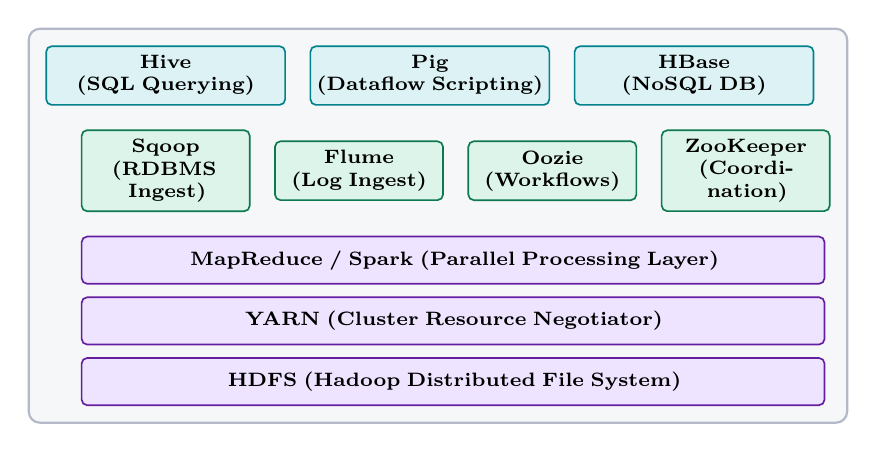
\begin{tikzpicture}[node distance=0.15cm and 0.2cm,
  sblock/.style={rectangle, draw=myteal, fill=hdrteal, text width=2.8cm,
    align=center, minimum height=0.7cm, font=\scriptsize\bfseries,
    rounded corners=2pt, line width=0.6pt},
  gblock/.style={rectangle, draw=mygreen, fill=hdrgreen, text width=1.9cm,
    align=center, minimum height=0.7cm, font=\scriptsize\bfseries,
    rounded corners=2pt, line width=0.6pt},
  rblock/.style={rectangle, draw=myred, fill=hdrred, text width=1.9cm,
    align=center, minimum height=0.7cm, font=\scriptsize\bfseries,
    rounded corners=2pt, line width=0.6pt},
  pblock/.style={rectangle, draw=mypurple, fill=hdrpurple, text width=9.2cm,
    align=center, minimum height=0.6cm, font=\scriptsize\bfseries,
    rounded corners=2pt, line width=0.6pt},
  bgbox/.style={draw=mgframe, fill=mygray, line width=0.8pt, rounded corners=4pt, inner sep=6pt}]

  % Application & Query layer
  \node[sblock] (hive) {Hive\\(SQL Querying)};
  \node[sblock, right=0.3cm of hive] (pig) {Pig\\(Dataflow Scripting)};
  \node[sblock, right=0.3cm of pig] (hbase) {HBase\\(NoSQL DB)};

  % Coordination, Ingestion, Workflows
  \node[gblock, below=0.3cm of hive] (sqoop) {Sqoop\\(RDBMS Ingest)};
  \node[gblock, right=0.3cm of sqoop] (flume) {Flume\\(Log Ingest)};
  \node[gblock, right=0.3cm of flume] (oozie) {Oozie\\(Workflows)};
  \node[gblock, right=0.3cm of oozie] (zk) {ZooKeeper\\(Coordination)};

  % Processing Frameworks Layer
  \node[pblock, below=0.3cm of sqoop.south west, anchor=north west] (mapred) {MapReduce / Spark (Parallel Processing Layer)};

  % Resource Management
  \node[pblock, below=0.15cm of mapred] (yarn) {YARN (Cluster Resource Negotiator)};

  % Storage Layer
  \node[pblock, below=0.15cm of yarn] (hdfs) {HDFS (Hadoop Distributed File System)};

  % Grouping background containers
  \begin{scope}[on background layer]
    \node[bgbox, fit=(hive) (pig) (hbase) (sqoop) (flume) (oozie) (zk) (mapred) (yarn) (hdfs)] (eco) {};
  \end{scope}

\end{tikzpicture}
\end{tcolorbox}

\subsection{Ecosystem Tools Overview}
\begin{itemize}[leftmargin=*, itemsep=3pt]
  \item \textbf{Sqoop:} A command-line tool designed for transferring bulk data between Apache Hadoop and structured datastores such as relational databases (e.g., MySQL, Oracle).
  \item \textbf{Flume:} A distributed, reliable, and available service for efficiently collecting, aggregating, and moving large amounts of streaming log data into HDFS.
  \item \textbf{ZooKeeper:} A centralized service for maintaining configuration information, naming, providing distributed synchronization, and group services.
  \item \textbf{Oozie:} A workflow scheduler system to manage Apache Hadoop jobs.
\end{itemize}

% ===============================================================================
\section{IBM Big Data Strategy and InfoSphere Tools}
% ===============================================================================

\subsection{IBM Big Data Strategy}
IBM's Big Data Strategy focuses on integrating enterprise-grade reliability, security, and governance standards with raw open-source Apache Hadoop. It is built on three core pillars:
\begin{enumerate}[leftmargin=*, itemsep=2pt]
  \item \textbf{Integration:} Bridging existing relational data warehouses (like IBM DB2) with unstructured Hadoop clusters.
  \item \textbf{Governance:} Providing trace tools for tracking data lineage and enforcing access security.
  \item \textbf{Acceleration:} Building analytical tools that execute queries faster than native MapReduce.
\end{enumerate}

\subsection{IBM InfoSphere BigInsights}
\begin{tcolorbox}[defbox, title={InfoSphere BigInsights}]
  \textbf{IBM InfoSphere BigInsights} was IBM's enterprise-grade distribution of Apache Hadoop. It combined the open-source Hadoop core with proprietary management tools, text analytics engines, and SQL querying features to simplify deployment and security.
\end{tcolorbox}

Key features of BigInsights include:
\begin{itemize}[leftmargin=*, itemsep=3pt]
  \item \textbf{SystemT:} A declarative, rule-based text analytics engine for extracting structure from unstructured documents.
  \item \textbf{Big SQL:} A low-latency, mass-parallel SQL querying engine that executes standard ANSI-SQL queries directly on HDFS.
\end{itemize}

\subsection{IBM Big Sheets}
\begin{tcolorbox}[defbox, title={Big Sheets}]
  \textbf{Big Sheets} is a browser-based, spreadsheet-like visualization and analysis interface built on top of BigInsights that allows business analysts to manipulate and analyze large datasets without writing complex Java MapReduce or Pig scripts.
\end{tcolorbox}

It utilizes a sheet model where users can apply formulas, filter rows, and build charts, which Big Sheets compiles into MapReduce jobs behind the scenes.

\newpage

% ═══════════════════════════════════════════════════════════════════════════════
% QUICK REVISION PAGE
% ═══════════════════════════════════════════════════════════════════════════════
\begin{center}
  {\large\bfseries\color{myred} Quick Revision --- Module 1}\\[3pt]
  {\small\color{mydark} Introduction to Big Data \& Hadoop Ecosystem $|$ OE-EC803B}
\end{center}
\noindent{\color{myred}\rule{\linewidth}{1.2pt}}
\vspace{8pt}

\begin{tcolorbox}[defbox, title={\textbf{One-Line Definitions}}]
\begin{itemize}[leftmargin=*, itemsep=3pt, topsep=0pt]
  \item \textbf{Structured Data:} Highly formatted tabular data with a pre-defined schema (e.g., SQL tables).
  \item \textbf{Big Data:} Datasets whose scale, speed, and diversity exceed the limits of storage and CPU architectures.
  \item \textbf{HDFS:} A block-structured distributed file system designed for running on commodity hardware.
  \item \textbf{YARN:} YARN is the Resource Negotiator layer that manages execution scheduling and CPU/RAM allocation.
  \item \textbf{Hadoop Streaming:} A utility allowing mappers/reducers to run as independent scripts using stdin/stdout.
  \item \textbf{Big Sheets:} A web-based spreadsheet interface for visualizing and exploring Big Data on Hadoop.
\end{itemize}
\end{tcolorbox}

\vspace{6pt}

\begin{tcolorbox}[exambox, title={\textbf{Frequently Asked / Viva Questions}}]
\begin{enumerate}[leftmargin=*, topsep=0pt, label=\textbf{Q\arabic*.}, itemsep=5pt]
  \item \Q{What are the differences between Semi-Structured and Unstructured data?}
        Semi-structured data lacks a formal database schema but contains internal tags or markers to represent structure (e.g., JSON, XML). Unstructured data has no predefined format or metadata identifiers (e.g., MP3 audio, video recordings, raw text).
        
  \item \Q{Detail the 5Vs of Big Data and why they matter.}
        Volume (scale of data), Velocity (generation speed), Variety (data formats), Veracity (data reliability), and Value (operational insights). They define whether a dataset requires Big Data tools instead of traditional relational databases.
        
  \item \Q{Why does RDBMS struggle with horizontal scaling?}
        RDBMS relies on maintaining ACID guarantees (Atomicity, Consistency, Isolation, Durability) across tables, which requires complex distributed locks. This creates severe performance bottlenecks when database tables are partitioned across different physical machines.
        
  \item \Q{What Google technologies inspired the creation of Apache Hadoop?}
        Google File System (GFS) published in 2003 inspired the creation of Hadoop Distributed File System (HDFS), and Google's MapReduce paper published in 2004 inspired Hadoop's MapReduce framework.
        
  \item \Q{How does Hadoop achieve data locality?}
        Hadoop schedules processing tasks directly on the physical node where the target HDFS data blocks are stored. This avoids copying large data files across the network, reducing network bandwidth bottlenecks.
        
  \item \Q{What is the difference between vertical scaling and horizontal scaling?}
        Vertical scaling (scale-up) involves adding resources (CPU, RAM) to a single machine, which has clear hardware limits. Horizontal scaling (scale-out) involves linking together multiple cheaper servers (commodity nodes) in a cluster to act as one.
        
  \item \Q{How does Hadoop Streaming handle communication between Java and other languages?}
        It spawns mappers/reducers as separate processes and communicates via standard I/O streams: input data is piped to the script's `stdin`, and the script writes output key-value pairs to its `stdout`.
        
  \item \Q{Explain the role of Sqoop and Flume in the Hadoop Ecosystem.}
        Sqoop is a tool used for bulk data transfer between relational databases (RDBMS) and HDFS. Flume is a distributed service designed for collecting and streaming log data into HDFS.
        
  \item \Q{What is the purpose of ZooKeeper in Hadoop clusters?}
        ZooKeeper acts as a central coordinator for maintaining cluster configuration, managing leader elections (e.g., Active NameNode election in HA clusters), and synchronizing distributed locks.
        
  \item \Q{What is IBM Big Sheets and who is its target user?}
        It is a web-based spreadsheet utility designed for business analysts to visualize and transform large datasets without writing MapReduce code. Behind the scenes, actions are converted into MapReduce tasks.
\end{enumerate}
\end{tcolorbox}

\vspace{6pt}

\begin{tcolorbox}[tikzbox, title={\textbf{Comparison Snapshot}}]
\textbf{Traditional RDBMS vs. Apache Hadoop:}\par\vspace{6pt}\noindent
{\renewcommand{\arraystretch}{1.4}%
\begin{tabularx}{\linewidth}{|B{3.2cm}|Y|Y|}
\hline
\textbf{Feature} & \textbf{Traditional RDBMS} & \textbf{Apache Hadoop} \\
\hline
Data Volume & Megabytes to Gigabytes (Gigabytes to Terabytes max) & Terabytes, Petabytes, and Exabytes \\
\hline
Data Variety & Only Structured (rigid tables) & Structured, Semi-Structured, and Unstructured \\
\hline
Schema Type & Schema-on-Write (rigorous validation) & Schema-on-Read (flexible query interpretation) \\
\hline
Access Paradigm & Interactive and Random (Low latency, high throughput) & Batch processing (High latency, massive scale throughput) \\
\hline
Scaling Type & Vertical (Adding bigger hardware) & Horizontal (Adding more commodity machines) \\
\hline
Cost per Gigabyte & High (requires enterprise servers and licensing) & Low (commodity hardware, open-source software) \\
\hline
\end{tabularx}}
\end{tcolorbox}


% -- Module 2 -----------------------------------------------------------------
\modulestart{2}{The Design of HDFS}

\section{The Design of HDFS}
% ===============================================================================

\begin{tcolorbox}[defbox, title={Hadoop Distributed File System (HDFS)}]
  \textbf{HDFS} is a distributed, block-structured file system designed to store very large files (typically Gigabytes to Petabytes) reliably across a cluster of commodity servers, providing high throughput access to application data using a write-once, read-many access pattern.
\end{tcolorbox}

Key design goals and assumptions include:
\begin{itemize}[leftmargin=*, itemsep=3pt]
  \item \textbf{Commodity Hardware Failure:} HDFS assumes hardware failures are common rather than exceptional. High fault tolerance is built in through automatic block replication.
  \item \textbf{Large Datasets:} Optimized to support large files. A single HDFS cluster can support millions of files.
  \item \textbf{Streaming Data Access:} Designed for batch processing rather than low-latency interactive access. Focuses on high data throughput over low latency.
  \item \textbf{Simple Coherency Model:} Uses a \textbf{write-once, read-many} pattern. Once a file is written, closed, and replicated, it cannot be modified inline. Appends are supported in later versions but random edits are not.
\end{itemize}

% ===============================================================================
\section{HDFS Concepts}
% ===============================================================================

\subsection{Blocks in HDFS}
Unlike standard physical hard drives where disk blocks are 512 bytes or 4KB, HDFS files are divided into large, discrete chunks called \textbf{Blocks}.

\begin{tcolorbox}[formulabox, title={HDFS Block Size Properties}]
  The standard block size in modern Hadoop distributions is \textbf{128MB} (or \textbf{256MB}).
  \begin{itemize}[leftmargin=*, noitemsep]
    \item \textbf{Reason for large blocks:} To minimize the cost of disk seeks. By making blocks large, the time taken to transfer data from disk to network is significantly larger than the time taken to seek to the start of the block.
    \item \textbf{Block Storage:} If a file is smaller than the block size (e.g., a 10MB file), it does not consume the full 128MB of physical space; it only uses 10MB on the local disk.
  \end{itemize}
\end{tcolorbox}

\subsection{NameNode, DataNode, and Secondary NameNode}
HDFS uses a master-slave architecture containing three key operational nodes:

\begin{tcolorbox}[tikzbox, title={HDFS Master-Slave Architecture}]
\centering
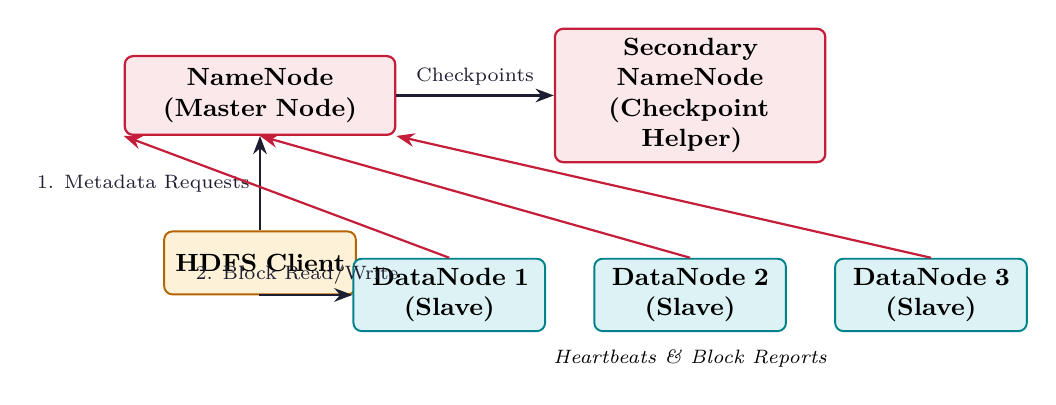
\begin{tikzpicture}[node distance=1.0cm and 1.5cm,
  mnode/.style={rectangle, draw=myred, fill=hdrred, text width=3.2cm, align=center, minimum height=1.0cm, font=\small\bfseries, rounded corners=3pt, line width=0.8pt},
  snode/.style={rectangle, draw=myteal, fill=hdrteal, text width=2.2cm, align=center, minimum height=0.9cm, font=\small\bfseries, rounded corners=3pt, line width=0.7pt},
  cnode/.style={rectangle, draw=myamber, fill=hdramber, text width=2.2cm, align=center, minimum height=0.8cm, font=\small\bfseries, rounded corners=3pt, line width=0.7pt}]

  % Nodes
  \node[mnode] (nn) {NameNode\\(Master Node)};
  \node[mnode, right=2.0cm of nn] (snn) {Secondary NameNode\\(Checkpoint Helper)};
  \node[cnode, below=1.2cm of nn] (client) {HDFS Client};

  \node[snode, below=1.2cm of snn] (dn2) {DataNode 2\\(Slave)};
  \node[snode, left=0.6cm of dn2] (dn1) {DataNode 1\\(Slave)};
  \node[snode, right=0.6cm of dn2] (dn3) {DataNode 3\\(Slave)};

  % Arrows
  \draw[arrow] (client) -- node[left, font=\scriptsize] {1. Metadata Requests} (nn);
  \draw[arrow] (client) |- node[pos=0.7, above, font=\scriptsize] {2. Block Read/Write} (dn1.west);
  \draw[arrow] (nn) -- node[above, font=\scriptsize] {Checkpoints} (snn);

  \draw[redarrow] (dn1.north) -- (nn.south west);
  \draw[redarrow] (dn2.north) -- (nn.south);
  \draw[redarrow] (dn3.north) -- (nn.south east);

  % Correct formatting for node text next to diagram
  \node[below=0.1cm of dn2, font=\scriptsize\itshape] {Heartbeats \& Block Reports};

\end{tikzpicture}
\end{tcolorbox}

\begin{itemize}[leftmargin=*, itemsep=4pt]
  \item \textbf{NameNode (Master):}
    \begin{itemize}[noitemsep]
      \item Manages the file system namespace (directories, files).
      \item Tracks the mapping of files to block IDs and their physical DataNode locations.
      \item Stores metadata in RAM for speed. Persists namespace changes in the \textbf{Edit Log} and holds the point-in-time filesystem state in \textbf{FSImage}.
    \end{itemize}
  \item \textbf{DataNode (Slave):}
    \begin{itemize}[noitemsep]
      \item Stores and retrieves HDFS data blocks on the local physical filesystem as directed by the NameNode.
      \item Sends periodic \textbf{Heartbeats} (confirming node availability) and \textbf{Block Reports} (listing all local blocks) to the NameNode.
    \end{itemize}
  \item \textbf{Secondary NameNode:}
    \begin{itemize}[noitemsep]
      \item It is NOT a backup/failover NameNode.
      \item It periodically merges the active \textbf{Edit Log} with the \textbf{FSImage} to prevent the Edit Log from growing too large. This process is called \textbf{Checkpointing}.
    \end{itemize}
\end{itemize}

% ===============================================================================
\section{HDFS Interfaces and Command Line Interface}
% ===============================================================================

\subsection{HDFS CLI (Command Line Interface)}
Users interact with HDFS files using standard terminal commands prefixed with `hdfs dfs` or `hadoop fs`.

\begin{tcolorbox}[examplebox, title={Common HDFS Terminal Commands}]
\renewcommand{\arraystretch}{1.3}
\begin{tabularx}{\linewidth}{|B{3.5cm}|Y|}
\hline
\textbf{Command} & \textbf{Description and Syntax} \\
\hline
`hdfs dfs -ls <path>` & Lists directory contents (analogous to Unix `ls`). \\
\hline
`hdfs dfs -put <src> <dest>` & Copies a local file from the client host into HDFS. \\
\hline
`hdfs dfs -get <src> <dest>` & Retrieves a file from HDFS and stores it locally. \\
\hline
`hdfs dfs -cat <path>` & Displays file contents directly on stdout. \\
\hline
`hdfs dfs -mkdir <path>` & Creates a new directory in HDFS. \\
\hline
`hdfs dfs -rm <path>` & Deletes a file or folder from HDFS. \\
\hline
\end{tabularx}
\end{tcolorbox}

\subsection{Hadoop File System Interfaces}
Hadoop supports programmatic interfaces to access HDFS files:
\begin{enumerate}[leftmargin=*, itemsep=3pt]
  \item \textbf{Java API:} The native interface. Uses the `org.apache.hadoop.fs.FileSystem` abstraction class, executing methods like `open()`, `create()`, and `delete()`.
  \item \textbf{WebHDFS REST API:} Provides complete read/write HTTP REST protocol endpoints to interact with HDFS from non-Java languages without loading fat native client libraries.
\end{enumerate}

% ===============================================================================
\section{HDFS Data Flow}
% ===============================================================================

Data flow operations in HDFS isolate the client from the details of block replication and network routing.

\subsection{Anatomy of a File Read}
\begin{enumerate}[leftmargin=*, itemsep=3pt]
  \item The Client calls `open()` on the `FileSystem` object (which is a `DistributedFileSystem` instance).
  \item The `DistributedFileSystem` calls the NameNode using RPC (Remote Procedure Call) to get the locations of the blocks for the first part of the file.
  \item The NameNode returns a list of DataNodes that have copies of those blocks, sorted by network proximity to the client.
  \item The client calls `read()` on the input stream (`FSDataInputStream`), which connects to the nearest DataNode.
  \item Once the end of the block is reached, `FSDataInputStream` closes the connection to that DataNode and opens a connection to the nearest DataNode for the next block, until reading is complete.
\end{enumerate}

\subsection{Anatomy of a File Write}
\begin{enumerate}[leftmargin=*, itemsep=3pt]
  \item The Client calls `create()` on the `DistributedFileSystem` object.
  \item The `DistributedFileSystem` makes an RPC call to the NameNode to create a new file in the filesystem namespace. The NameNode checks permissions and verifies the path does not already exist.
  \item The client writes data to the output stream (`FSDataOutputStream`), which splits it into packets and writes them to an internal queue called the \textbf{Data Queue}.
  \item The \textbf{Data Streamer} requests the NameNode to allocate new blocks and choose DataNodes to store replicas (typically 3 DataNodes for a replication factor of 3).
  \item A pipeline is formed between the selected DataNodes (e.g., DataNode A $\rightarrow$ DataNode B $\rightarrow$ DataNode C). The Data Streamer streams packets to the first DataNode, which passes them to the second, which passes them to the third.
  \item When the client finishes writing data, it calls `close()`, which flushes all remaining packets to the DataNodes and contacts the NameNode to commit the file creation.
\end{enumerate}

% ===============================================================================
\section{Data Ingestion: Sqoop and Flume}
% ===============================================================================

To analyze data in Hadoop, it must first be ingested from external sources.

\subsection{Apache Sqoop}
\begin{tcolorbox}[defbox, title={Apache Sqoop (SQL to Hadoop)}]
  \textbf{Sqoop} is a tool designed to transfer bulk data between relational databases (RDBMS) and the Hadoop Ecosystem (HDFS, Hive, HBase). It translates import and export commands into MapReduce jobs to execute parallel data transfers.
\end{tcolorbox}

\begin{itemize}[leftmargin=*, itemsep=3pt]
  \item \textbf{Import Mechanism:} Reads rows from an RDBMS table, generates a MapReduce job where mappers read data in parallel using SQL boundaries, and writes the output files to HDFS.
  \item \textbf{Export Mechanism:} Reads files from HDFS and inserts records into a target database table in parallel using database insert statements.
\end{itemize}

\subsection{Apache Flume}
\begin{tcolorbox}[defbox, title={Apache Flume}]
  \textbf{Flume} is a distributed service designed for efficiently collecting, aggregating, and moving large amounts of streaming log data (such as web server logs or social media streams) into HDFS.
\end{tcolorbox}

An active Flume agent consists of three main components:
\begin{enumerate}[leftmargin=*, itemsep=3pt]
  \item \textbf{Source:} Receives event data from external generators (e.g., Syslog, HTTP) and pushes it into one or more channels.
  \item \textbf{Channel:} A passive store that buffers the events until they are consumed by a sink (can be in-memory for speed or file-based for durability).
  \item \textbf{Sink:} Removes events from the channel and stores them in an external repository like HDFS or HBase.
\end{enumerate}

% ===============================================================================
\section{Hadoop Archives (HAR)}
% ===============================================================================

Every file, directory, and block in HDFS occupies about 150 bytes of memory in the NameNode's RAM. If a cluster stores millions of small files (smaller than the block size), the NameNode RAM becomes a performance bottleneck.

\begin{tcolorbox}[defbox, title={Hadoop Archives (HAR)}]
  \textbf{Hadoop Archives (HAR)} are file archiving tools that pack HDFS files into larger archive files (`.har` files) to reduce the metadata overhead in the NameNode, while still allowing applications to access the individual files transparently.
\\
A `.har` archive contains index files listing the metadata and a set of part files containing the concatenated data blocks.
\end{tcolorbox}

% ===============================================================================
\section{Hadoop I/O: Compression, Serialization, and File Structures}
% ===============================================================================

\subsection{Compression Codecs}
Hadoop supports data compression to save storage space and reduce network and disk I/O overhead.

\par\vspace{6pt}\noindent
{\renewcommand{\arraystretch}{1.4}%
\begin{tabularx}{\linewidth}{|B{2.5cm}|Y|Y|Y|}
\hline
\textbf{Codec} & \textbf{Algorithm} & \textbf{Splittable?} & \textbf{Key Characteristics} \\
\hline
\textbf{Gzip} & DEFLATE & No & High compression ratio, slow speed. \\
\hline
\textbf{Bzip2} & Burrows-Wheeler & Yes & Extremely high compression ratio, very slow. \\
\hline
\textbf{LZO} & LZO & Yes (if indexed) & Fast compression and decompression. \\
\hline
\textbf{Snappy} & Snappy & No & Very fast speed, moderate compression. \\
\hline
\end{tabularx}}

\textbf{Why Splittability Matters:} If a compression format is splittable, MapReduce can split the file and process different portions on separate mappers in parallel. If it is not splittable, a single mapper must process the entire file sequentially, breaking the parallel execution model.

\subsection{Serialization}
\begin{tcolorbox}[defbox, title={Serialization}]
  \textbf{Serialization} is the process of converting structured objects into a stream of bytes for transmission over a network or storage on disk. \textbf{Deserialization} is the reverse process of turning a byte stream back into live runtime objects.
\end{tcolorbox}

Hadoop does not use standard Java serialization because it is too bloated. Instead, it defines its own lightweight protocols:
\begin{itemize}[leftmargin=*, itemsep=3pt]
  \item \textbf{Writable Interface:} Mappers and Reducers exchange keys and values implementing the \textbf{Writable} interface. It provides high-speed serialization using compact byte formats.
  \item \textbf{Avro:} A language-neutral serialization system that stores data schemas in JSON files, making it easy for different languages (Java, C++, Python) to share data records.
\end{itemize}

\subsection{File-Based Data Structures}
Hadoop provides specialized container files for binary data:
1. \textbf{SequenceFile:} A persistent, binary container file format for storing key-value pairs. It supports compression and includes \textbf{sync markers} to allow MapReduce splits.
2. \textbf{MapFile:} A sorted version of \textbf{SequenceFile} that contains an index file (`/index`) alongside the data file (`/data`) to allow fast random access by key.

\newpage

% ═══════════════════════════════════════════════════════════════════════════════
% QUICK REVISION PAGE
% ═══════════════════════════════════════════════════════════════════════════════
\begin{center}
  {\large\bfseries\color{myred} Quick Revision --- Module 2}\\[3pt]
  {\small\color{mydark} HDFS Concepts, CLI \& I/O Architectures $|$ OE-EC803B}
\end{center}
\noindent{\color{myred}\rule{\linewidth}{1.2pt}}
\vspace{8pt}

\begin{tcolorbox}[defbox, title={\textbf{One-Line Definitions}}]
\begin{itemize}[leftmargin=*, itemsep=3pt, topsep=0pt]
  \item \textbf{DataNode:} A slave node in HDFS that physically stores data blocks on local disks.
  \item \textbf{Secondary NameNode:} A helper node that periodically merges Edit Logs with FSImage (Checkpointing).
  \item \textbf{Splittability:} The property of a file format/codec that allows it to be split into chunks for parallel MapReduce execution.
  \item \textbf{SequenceFile:} A persistent binary file format that stores sequential key-value data.
  \item \textbf{Avro:} A serialization framework using JSON-defined schemas for cross-language data exchanges.
\end{itemize}
\end{tcolorbox}

\vspace{6pt}

\begin{tcolorbox}[exambox, title={\textbf{Frequently Asked / Viva Questions}}]
\begin{enumerate}[leftmargin=*, topsep=0pt, label=\textbf{Q\arabic*.}, itemsep=5pt]
  \item \Q{Why does HDFS use a large block size (e.g., 128MB)?}
        Large block sizes minimize the disk seek overhead. Since disk seeks take several milliseconds, setting the block size to 128MB ensures that the disk transfer time (reading data) is significantly larger than the seek time, maximizing throughput.
        
  \item \Q{How does checkpointing work in the Secondary NameNode?}
        The Secondary NameNode fetches the active Edit Log and current FSImage from the NameNode, merges them in memory to generate a new FSImage checkpoint, and sends it back to the NameNode. This keeps the Edit Log from growing too large.
        
  \item \Q{Describe the HDFS replication strategy (Rack Awareness).}
        For a replication factor of 3: HDFS places the first replica on a node in the local rack, the second replica on a different node in a remote rack, and the third replica on a different node within that same remote rack. This balances fault tolerance and write latency.
        
  \item \Q{What happens if a DataNode fails in an HDFS cluster?}
        If a DataNode fails to send Heartbeats to the NameNode for a timeout period (typically 10 minutes), the NameNode marks it as dead. It scans the metadata, identifies all blocks stored on the failed node, and schedules copies of those blocks to other nodes to restore the replication factor.
        
  \item \Q{What is the difference between client-side reads and client-side writes in HDFS?}
        During a read, the client only queries the NameNode for block locations and reads directly from the nearest DataNode. During a write, the client streams packets to a pipeline of DataNodes, which replicate data to each other while sending ACKs back.
        
  \item \Q{Explain the agent architecture of Apache Flume.}
        A Flume agent consists of a \textbf{Source} (ingests raw logs from external clients), a \textbf{Channel} (buffers events in memory or on disk), and a \textbf{Sink} (drains the channel to write files into HDFS).
        
  \item \Q{Why are Hadoop Archives (HAR) used for small files?}
        Each file in HDFS consumes 150 bytes of metadata in the NameNode's RAM. Millions of small files can exhaust NameNode memory. HAR bundles these files into larger archive containers, reducing the total metadata footprint.
        
  \item \Q{Which compression codecs are splittable in MapReduce?}
        Bzip2 is natively splittable. LZO is splittable if an index is built for it. Gzip and Snappy are not splittable.
        
  \item \Q{Why did Hadoop develop its own Writable serialization system instead of using Java Serialization?}
        Java's default serialization is too heavy, storing class names, parent classes, and metadata along with the data. Hadoop's Writable system is lightweight, compact, and optimized for high-speed network transmission.
        
  \item \Q{What is the difference between a SequenceFile and a MapFile?}
        A SequenceFile stores binary key-value pairs sequentially. A MapFile is a directory containing a sorted SequenceFile (`/data`) and an index file (`/index`) that maps keys to offsets for random lookups.
\end{enumerate}
\end{tcolorbox}

\vspace{6pt}

\begin{tcolorbox}[tikzbox, title={\textbf{Comparison Snapshot}}]
\textbf{NameNode vs. DataNode:}\par\vspace{6pt}\noindent
{\renewcommand{\arraystretch}{1.4}%
\begin{tabularx}{\linewidth}{|B{3.2cm}|Y|Y|}
\hline
\textbf{Feature} & \textbf{NameNode} & \textbf{DataNode} \\
\hline
Role & Master Node & Slave Node \\
\hline
Primary Data stored & File metadata, namespace mapping, block locations & Actual data blocks (replicated payload) \\
\hline
Storage Media & System RAM (for speed) & Physical Hard Drive / SSD \\
\hline
Hardware requirements & Enterprise grade (high RAM capacity) & Commodity servers (large storage disks) \\
\hline
Quantity in Cluster & Active/Standby pair (HA configurations) & Thousands of nodes in large clusters \\
\hline
Failure Impact & High (cluster down if master fails without HA) & Low (re-replicated from other nodes) \\
\hline
\end{tabularx}}
\end{tcolorbox}


% -- Module 3 -----------------------------------------------------------------
\modulestart{3}{Anatomy of a MapReduce Job Run}

\section{Anatomy of a MapReduce Job Run}
% ===============================================================================

MapReduce execution is divided into MapReduce 1 (Classic MapReduce) and MapReduce 2 (built on YARN).

\begin{tcolorbox}[defbox, title={Classic MapReduce vs. YARN}]
  \begin{itemize}[leftmargin=*, noitemsep]
    \item \textbf{MapReduce 1 (Classic):} Job execution was coordinated by a single master process called the \textbf{JobTracker}, which scheduled tasks and monitored slaves called \textbf{TaskTrackers}.
    \item \textbf{YARN (MapReduce 2):} Divides the resource management and job scheduling functions into separate daemons: a global \textbf{ResourceManager} and application-specific \textbf{ApplicationMasters}.
  \end{itemize}
\end{tcolorbox}

\subsection{YARN Runtime Job Execution Steps}
YARN runs MapReduce jobs using several steps:
\begin{enumerate}[leftmargin=*, itemsep=3pt]
  \item \textbf{Job Submission:} The Client program calls `submitJob()` on the Job object, requesting a new Application ID from the ResourceManager.
  \item \textbf{Application Master Launch:} The ResourceManager allocates a \textbf{Container} (allocated CPU/RAM limit) on a NodeManager and starts the \textbf{ApplicationMaster} process there.
  \item \textbf{Resource Allocation:} The ApplicationMaster registers with the ResourceManager and requests containers across NodeManagers to host the Map and Reduce tasks.
  \item \textbf{Task Execution:} The ApplicationMaster contacts the NodeManagers to launch the tasks within the allocated containers. Tasks retrieve data blocks from local HDFS DataNodes, process them, and write outputs locally.
\end{enumerate}

\begin{tcolorbox}[tikzbox, title={YARN Resource Management Layout}]
\centering
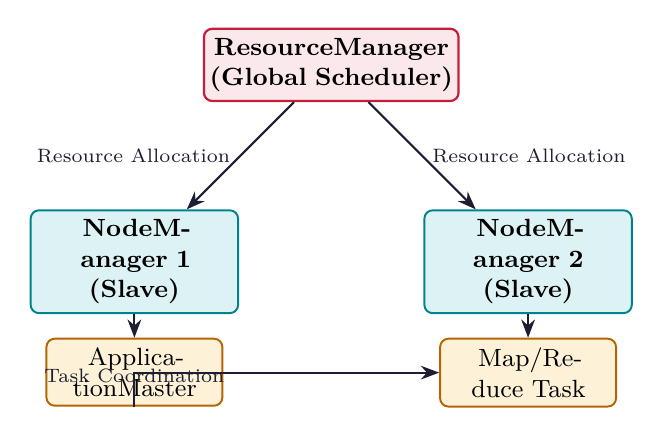
\begin{tikzpicture}[node distance=0.8cm and 1.2cm,
  rmnode/.style={rectangle, draw=myred, fill=hdrred, text width=3.0cm, align=center, minimum height=0.85cm, font=\small\bfseries, rounded corners=3pt, line width=0.8pt},
  nmnode/.style={rectangle, draw=myteal, fill=hdrteal, text width=2.4cm, align=center, minimum height=0.8cm, font=\small\bfseries, rounded corners=3pt, line width=0.7pt},
  cnode/.style={rectangle, draw=myamber, fill=hdramber, text width=2.0cm, align=center, minimum height=0.75cm, font=\small, rounded corners=3pt, line width=0.7pt},
  lnarrow/.style={-Stealth, thick, color=mydark}]

  % Nodes
  \node[rmnode] (rm) at (0,2.5) {ResourceManager\\(Global Scheduler)};
  \node[nmnode] (nm1) at (-2.5,0) {NodeManager 1\\(Slave)};
  \node[nmnode] (nm2) at (2.5,0) {NodeManager 2\\(Slave)};

  \node[cnode, below=0.3cm of nm1] (am) {ApplicationMaster};
  \node[cnode, below=0.3cm of nm2] (task) {Map/Reduce Task};

  % Connections
  \draw[lnarrow] (rm) -- node[left, font=\scriptsize] {Resource Allocation} (nm1);
  \draw[lnarrow] (rm) -- node[right, font=\scriptsize] {Resource Allocation} (nm2);
  \draw[lnarrow] (nm1) -- (am);
  \draw[lnarrow] (nm2) -- (task);
  \draw[lnarrow] (am) |- node[pos=0.2, above, font=\scriptsize] {Task Coordination} (task.west);

\end{tikzpicture}
\end{tcolorbox}

% ===============================================================================
\section{Failures in YARN}
% ===============================================================================

Distributed systems must tolerate node and task failures gracefully.

\subsection{Task Failure}
A Map or Reduce task can fail due to runtime Java exceptions or JVM crashes.
\begin{itemize}[leftmargin=*, itemsep=3pt]
  \item \textbf{Detection:} The NodeManager detects that the task JVM exited with a non-zero code and reports the failure back to the ApplicationMaster.
  \item \textbf{Resolution:} The ApplicationMaster reschedules the task on a different NodeManager. It will retry the task up to 4 times (default limit) before marking the entire job as failed.
\end{itemize}

\subsection{NodeManager Failure}
\begin{itemize}[leftmargin=*, itemsep=3pt]
  \item \textbf{Detection:} The NodeManager sends heartbeats to the ResourceManager. If heartbeats stop (typically for 10 minutes), the ResourceManager marks the NodeManager as dead.
  \item \textbf{Resolution:} The ResourceManager notifies the active ApplicationMasters. The ApplicationMasters reschedule all tasks (both active and completed map tasks) that were running on the failed NodeManager, since their local map outputs are no longer accessible.
\end{itemize}

\subsection{ResourceManager / ApplicationMaster Failure}
\begin{itemize}[leftmargin=*, itemsep=3pt]
  \item \textbf{ApplicationMaster Failure:} The ResourceManager detects the loss of heartbeat from the ApplicationMaster and starts a new container to launch a fresh ApplicationMaster instance.
  \item \textbf{ResourceManager Failure:} This is a single point of failure (SPOF). It is resolved by running active-standby ResourceManagers using ZooKeeper to manage failover and state replication.
\end{itemize}

% ===============================================================================
\section{Job Scheduling}
% ===============================================================================

YARN supports three primary job scheduling engines:

\begin{enumerate}[leftmargin=*, itemsep=4pt]
  \item \textbf{FIFO (First-In, First-Out) Scheduler:} Allocates resources strictly based on job submission order. A large, slow job at the head of the queue will block all subsequent small jobs.
  \item \textbf{Capacity Scheduler:} Allocates distinct organizational queues, where each queue is guaranteed a fixed percentage of cluster capacity (e.g., Queue A gets 40\%, Queue B gets 60\%). If a queue has free space, it can temporarily lend it to other queues.
  \item \textbf{Fair Scheduler:} Dynamically balances resources so that all running jobs get an equal share of cluster capacity over time. When a single job runs, it uses 100\% of the cluster; when a second job is submitted, YARN re-allocates 50\% of the resources to it.
\end{enumerate}

% ===============================================================================
\section{Shuffle and Sort Phase}
% ===============================================================================

\begin{tcolorbox}[defbox, title={The Shuffle and Sort}]
  The \textbf{Shuffle and Sort} is the core transport layer of MapReduce that routes intermediate key-value outputs from mappers to the correct reducers, guaranteeing that all values associated with a specific key are grouped and delivered to the same reducer in sorted order.
\end{tcolorbox}

The shuffle process runs across the map and reduce stages:

\subsection{Map Side Execution Details}
\begin{enumerate}[leftmargin=*, itemsep=3pt]
  \item \textbf{Circular Buffer:} The Map task writes outputs to an in-memory circular RAM buffer (default size: 100MB).
  \item \textbf{Spilling:} When the buffer fill percentage reaches a threshold (default: 80\%), a background thread wakes up to spill the data to the local disk.
  \item \textbf{Partitioning:} Before writing to disk, the thread divides the key-value records into partitions based on the target Reducer ID (using \texttt{HashPartitioner} by default: \texttt{(key.hashCode() \& Integer.MAX\_VALUE) \% numReducers}).
  \item \textbf{Sorting:} Within each partition, the keys are sorted in memory using a quicksort algorithm.
  \item \textbf{Combining:} If a local `Combiner` (mini-reducer) is defined, it runs on the sorted partition records before writing to disk to reduce data volume.
  \item \textbf{Merging:} When the Map task finishes, all local spill files are merged and sorted to create a single partitioned and sorted output file on the local node.
\end{enumerate}

\subsection{Reduce Side Execution Details}
\begin{enumerate}[leftmargin=*, itemsep=3pt]
  \item \textbf{Copy Phase:} The Reducer tasks have copier threads that fetch their respective partition files from all mapper nodes over HTTP (using the MapOutputServlet).
  \item \textbf{Merge Phase:} As files are copied, background threads merge and sort the incoming data in passes.
  \item \textbf{Reduce Phase:} The sorted key-value pairs are fed to the `reduce()` method line-by-line.
\end{enumerate}

% ===============================================================================
\section{MapReduce Types and Formats}
% ===============================================================================

MapReduce enforces strict type checking using serialization wrappers (e.g., `Text` for Java String, `IntWritable` for Integer).

\subsection{Input Splits and InputFormat}
\begin{itemize}[leftmargin=*, itemsep=3pt]
  \item \textbf{InputSplit:} A chunk of HDFS data processed by a single mapper. Typically equals the HDFS block size (128MB).
  \item \textbf{InputFormat:} Validates the input files and defines how to split them. It spawns the \textbf{RecordReader} to convert split byte streams into key-value records.
\end{itemize}

\par\vspace{6pt}\noindent
{\renewcommand{\arraystretch}{1.4}%
\begin{tabularx}{\linewidth}{|B{3.2cm}|Y|Y|}
\hline
\textbf{InputFormat} & \textbf{Key Type} & \textbf{Value Type} \\
\hline
`TextInputFormat` & `LongWritable` (Byte offset of line) & `Text` (Content of the text line) \\
\hline
`KeyValueTextInputFormat` & `Text` (Text before separator) & `Text` (Text after separator) \\
\hline
`SequenceFileInputFormat` & User-defined binary key type & User-defined binary value type \\
\hline
\end{tabularx}}

% ===============================================================================
\section{Advanced MapReduce Features}
% ===============================================================================

\subsection{Counters}
Counters are used to collect statistics about MapReduce jobs (e.g., counting empty records or corrupt lines).
\begin{itemize}[leftmargin=*, itemsep=3pt]
  \item \textbf{Built-in Counters:} Automatically populated by YARN (e.g., Map Input Records, Bytes Written).
  \item \textbf{User-Defined Counters:} Programmed in Java using enums: \texttt{context.getCounter(MyEnum.CORRUPT\_ROWS).increment(1)}.
\end{itemize}

\subsection{Joins in MapReduce}
When combining datasets (e.g., Customers and Orders tables), two join strategies are used:

\par\vspace{6pt}\noindent
{\renewcommand{\arraystretch}{1.4}%
\begin{tabularx}{\linewidth}{|B{3.0cm}|Y|Y|}
\hline
\textbf{Feature} & \textbf{Map-Side Join} & \textbf{Reduce-Side Join} \\
\hline
Execution Phase & Done completely inside the Mapper. & Done inside the Reducer. \\
\hline
Prerequisites & Datasets must be sorted and bucketed by the join key. One dataset must be small enough to fit in memory. & None. General-purpose join. \\
\hline
Shuffle Overhead & Zero shuffle overhead (fastest). & Heavy network shuffle of all records. \\
\hline
Data Volume Limit & Limited by Mapper node RAM. & Unlimited (handles massive datasets). \\
\hline
\end{tabularx}}

\newpage

% ═══════════════════════════════════════════════════════════════════════════════
% QUICK REVISION PAGE
% ═══════════════════════════════════════════════════════════════════════════════
\begin{center}
  {\large\bfseries\color{myred} Quick Revision --- Module 3}\\[3pt]
  {\small\color{mydark} MapReduce Internals, YARN Scheduler \& Joins $|$ OE-EC803B}
\end{center}
\noindent{\color{myred}\rule{\linewidth}{1.2pt}}
\vspace{8pt}

\begin{tcolorbox}[defbox, title={\textbf{One-Line Definitions}}]
\begin{itemize}[leftmargin=*, itemsep=3pt, topsep=0pt]
  \item \textbf{ApplicationMaster:} A per-application YARN process that negotiates resources and coordinates task runs.
  \item \textbf{Container:} A logical YARN resource allocation containing CPU cores and RAM limits on a NodeManager.
  \item \textbf{Speculative Execution:} A task execution strategy that runs duplicate copies of slow-running tasks in parallel to minimize job latency.
  \item \textbf{Combiner:} A local semi-reducer that aggregates Map outputs locally before the network shuffle.
  \item \textbf{RecordReader:} A helper class that translates raw HDFS data splits into structured key-value objects.
\end{itemize}
\end{tcolorbox}

\vspace{6pt}

\begin{tcolorbox}[exambox, title={\textbf{Frequently Asked / Viva Questions}}]
\begin{enumerate}[leftmargin=*, topsep=0pt, label=\textbf{Q\arabic*.}, itemsep=5pt]
  \item \Q{What are the differences between MapReduce 1 (Classic) and YARN?}
        In MapReduce 1, the JobTracker was responsible for both resource management and task scheduling, creating scalability bottlenecks. YARN decouples these tasks, using a global \textbf{ResourceManager} for cluster resource allocation and a per-job \textbf{ApplicationMaster} for scheduling.
        
  \item \Q{Detail the spilling process on the Map side.}
        Mappers write outputs to a 100MB circular buffer. When the buffer is 80\% full, a background thread locks the data, partitions it based on Reducer IDs, sorts it by key, runs the optional combiner, and writes (spills) the sorted partition files to local disk.
        
  \item \Q{How does the Fair Scheduler distribute cluster resources?}
        The Fair Scheduler divides resources dynamically so that all active jobs receive an equal share of CPU and RAM over time. If only one job runs, it uses the entire cluster. When a second job starts, YARN re-allocates 50\% of the resources to it.
        
  \item \Q{Why does a NodeManager failure force mappers to rerun, but not reducers?}
        Mappers store their intermediate partition outputs on local disks, so if the mapper's node dies, those files are lost. Reducers write their final outputs directly to replicated HDFS blocks, which remain accessible even if a NodeManager fails.
        
  \item \Q{What is the difference between TextInputFormat and KeyValueTextInputFormat?}
        `TextInputFormat` treats the line offset as the key (`LongWritable`) and the line text as the value (`Text`). `KeyValueTextInputFormat` splits each line at a separator character (like a tab) to define both the key and the value as `Text`.
        
  \item \Q{Explain Map-side Joins and their memory constraints.}
        A Map-side Join joins datasets inside the Mapper without a network shuffle. It requires that all datasets are pre-sorted and bucketed by the join key, and one of the datasets must be small enough to load entirely into the mapper's JVM memory.
        
  \item \Q{Why does speculative execution not run for tasks with side effects?}
        Speculative execution launches duplicate tasks. If a task writes to an external database, running duplicate tasks would cause duplicate writes. Therefore, speculative execution should be disabled for tasks with external side effects.
        
  \item \Q{What is the purpose of sync markers in a SequenceFile?}
        Sync markers are special byte sequences placed periodically in a SequenceFile. They allow MapReduce to split the file at arbitrary boundaries, as the RecordReader can seek to a random position and scan forward to find the next sync marker.
        
  \item \Q{How does secondary sorting work in MapReduce?}
        It allows sorting the values associated with a key. It is implemented by creating a composite key (comprising the natural key and the secondary sort value), partitioning by the natural key, and sorting by the composite key.
        
  \item \Q{What does the HashPartitioner do?}
        It computes the partition index for a mapper output key: \texttt{(key.hashCode() \& Integer.MAX\_VALUE) \% numReducers}. This ensures that all records with the same key are routed to the same Reducer ID.
\end{enumerate}
\end{tcolorbox}

\vspace{6pt}

\begin{tcolorbox}[tikzbox, title={\textbf{Comparison Snapshot}}]
\textbf{Capacity Scheduler vs. Fair Scheduler:}\par\vspace{6pt}\noindent
{\renewcommand{\arraystretch}{1.4}%
\begin{tabularx}{\linewidth}{|B{3.2cm}|Y|Y|}
\hline
\textbf{Feature} & \textbf{Capacity Scheduler} & \textbf{Fair Scheduler} \\
\hline
Primary Design Goal & Organization queues with guaranteed shares & Dynamic, equal sharing of cluster resources \\
\hline
Queue Configuration & Strict hierarchical queues (e.g., Sales, Dev) & Simple resource shares per running application \\
\hline
Resource Loaning & Queues can borrow unused capacity from others & Idle capacity is divided among active jobs \\
\hline
Preemption & Not supported (waits for tasks to end) & Supported (reclaims resources by killing tasks) \\
\hline
Use Case & Multi-tenant corporate cluster with fixed budgets & Ad-hoc environments with variable workloads \\
\hline
\end{tabularx}}
\end{tcolorbox}


% -- Module 4 -----------------------------------------------------------------
\modulestart{4}{Apache Pig}

\section{Apache Pig}
% ===============================================================================

\begin{tcolorbox}[defbox, title={Apache Pig}]
  \textbf{Apache Pig} is a high-level dataflow platform designed for processing large datasets on Hadoop. It provides a procedural dataflow programming language called \textbf{Pig Latin}, which compiles scripts into sequences of MapReduce jobs executed across a YARN cluster.
\end{tcolorbox}

\subsection{Execution Modes and Components}
\begin{itemize}[leftmargin=*, itemsep=3pt]
  \item \textbf{Local Mode:} Runs in a single JVM using the local filesystem. Excellent for testing and debugging.
  \item \textbf{MapReduce Mode:} Translates scripts into MapReduce jobs and executes them on an active Hadoop cluster.
  \item \textbf{Grunt Shell:} The interactive command-line shell used to type Pig Latin statements.
  \item \textbf{UDF (User Defined Functions):} Allows developers to write custom processing logic in Java, Python, or JavaScript when Pig's built-in operators are insufficient.
\end{itemize}

\subsection{Pig Latin Data Model}
Pig Latin supports both simple types (e.g., `int`, `chararray`) and complex nested types:
\begin{itemize}[leftmargin=*, itemsep=3pt]
  \item \textbf{Atom:} Any single value stored as a string (e.g., `'Biraj'`, `45`).
  \item \textbf{Tuple:} An ordered set of fields (e.g., `(Biraj, 22, CGEC)`).
  \item \textbf{Bag:} A collection of tuples (e.g., `{(Biraj, 22), (Amit, 23)}`).
  \item \textbf{Map:} A set of key-value pairs (e.g., \texttt{['name'\#'Biraj', 'age'\#'22']}).
\end{itemize}

\subsection{Core Processing Operators}
\begin{itemize}[leftmargin=*, itemsep=3pt]
  \item `LOAD`: Ingests data from HDFS files.
  \item `FILTER`: Selects tuples from a relation based on conditions.
  \item `FOREACH ... GENERATE`: Transforms data columns.
  \item `GROUP`: Collects tuples sharing a key into a bag.
  \item `JOIN`: Joins relations based on matching keys.
\end{itemize}

% ===============================================================================
\section{Apache Hive}
% ===============================================================================

\begin{tcolorbox}[defbox, title={Apache Hive}]
  \textbf{Apache Hive} is a data warehouse software system built on top of Apache Hadoop that provides data summarization, ad-hoc querying, and analysis of large datasets stored in HDFS. It provides an SQL-like query language called \textbf{HiveQL}.
\end{tcolorbox}

\subsection{Hive Architecture}
Hive translates SQL-like HiveQL statements into MapReduce, Tez, or Spark jobs.

\begin{tcolorbox}[tikzbox, title={Hive System Architecture}]
\centering
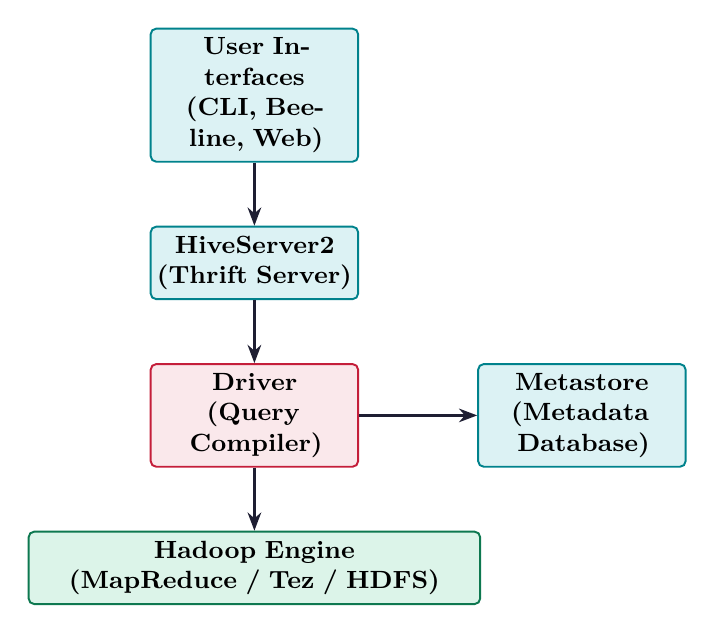
\begin{tikzpicture}[node distance=0.7cm and 1.0cm,
  bblock/.style={rectangle, draw=myteal, fill=hdrteal, text width=2.4cm, align=center, minimum height=0.8cm, font=\small\bfseries, rounded corners=2pt, line width=0.7pt},
  rblock/.style={rectangle, draw=myred, fill=hdrred, text width=2.4cm, align=center, minimum height=0.8cm, font=\small\bfseries, rounded corners=2pt, line width=0.7pt},
  gblock/.style={rectangle, draw=mygreen, fill=hdrgreen, text width=5.5cm, align=center, minimum height=0.75cm, font=\small\bfseries, rounded corners=2pt, line width=0.7pt}]

  % Nodes
  \node[bblock] (ui) {User Interfaces\\(CLI, Beeline, Web)};
  \node[bblock, below=0.8cm of ui] (hs2) {HiveServer2\\(Thrift Server)};

  \node[rblock, below=0.8cm of hs2] (driver) {Driver\\(Query Compiler)};
  \node[bblock, right=1.5cm of driver] (ms) {Metastore\\(Metadata Database)};
  \node[gblock, below=0.8cm of driver] (hadoop) {Hadoop Engine\\(MapReduce / Tez / HDFS)};

  % Arrows
  \draw[arrow] (ui) -- (hs2);
  \draw[arrow] (hs2) -- (driver);
  \draw[arrow] (driver) -- (ms);
  \draw[arrow] (driver) -- (hadoop);

\end{tikzpicture}
\end{tcolorbox}

\begin{itemize}[leftmargin=*, itemsep=3pt]
  \item \textbf{Metastore:} A relational database (typically MySQL or Derby) that stores schema definitions, column details, and partition metadata.
  \item \textbf{HiveServer2:} The execution endpoint allowing remote JDBC/ODBC clients to submit queries.
\end{itemize}

\subsection{Managed vs. External Tables}
Hive supports two types of tables to control data ownership:

\par\vspace{6pt}\noindent
{\renewcommand{\arraystretch}{1.4}%
\begin{tabularx}{\linewidth}{|B{3.2cm}|Y|Y|}
\hline
\textbf{Feature} & \textbf{Managed Table (Internal)} & \textbf{External Table} \\
\hline
Data Ownership & Hive owns both the metadata and the data. & Hive only owns the metadata. \\
\hline
Storage Path & Default directory: `/user/hive/warehouse/` & User-defined HDFS location. \\
\hline
`DROP TABLE` Impact & Deletes both the HDFS data and metadata. & Deletes metadata; HDFS data remains intact. \\
\hline
Use Case & Temporary tables, internal application data. & Sharing datasets with Spark, Pig, or MapReduce. \\
\hline
\end{tabularx}}

\subsection{Partitioning vs. Bucketing}
Hive optimizes query performance using two layout patterns:

\begin{tcolorbox}[formulabox, title={Partitioning vs. Bucketing Properties}]
  \begin{itemize}[leftmargin=*, noitemsep]
    \item \textbf{Partitioning:} Divides a table into subdirectories based on column values (e.g., `/country=IN/`, `/country=US/`). It significantly reduces query search space by pruning directories.
    \item \textbf{Bucketing:} Distributes table rows into a fixed number of files (buckets) based on a hash function of a column (e.g., `hash(userID) \% numBuckets`). It speeds up joins and sampling on high-cardinality columns.
  \end{itemize}
\end{tcolorbox}

% ===============================================================================
\section{Apache HBase}
% ===============================================================================

\begin{tcolorbox}[defbox, title={Apache HBase}]
  \textbf{Apache HBase} is a distributed, column-oriented, multi-dimensional, NoSQL database built on top of HDFS, modeled after Google's Bigtable, designed to provide random, real-time read/write access to billions of rows and columns.
\end{tcolorbox}

\subsection{HBase Architecture and Components}
HBase achieves horizontal scale using master-slave coordinators:
\begin{itemize}[leftmargin=*, itemsep=3pt]
  \item \textbf{HMaster:} Coordinates the cluster, assigns regions to RegionServers, and handles schema updates.
  \item \textbf{RegionServer:} Manages a set of dynamic table splits called \textbf{Regions}. Handles client read/write requests directly.
  \item \textbf{Write-Ahead Log (WAL):} A local disk file where writes are written first for durability before committing to RAM.
  \item \textbf{MemStore:} The write buffer in RAM. Writes are accumulated here first.
  \item \textbf{HFile:} The physical file format stored on HDFS. When a MemStore fills up (flushes), its contents are written to disk as an HFile.
\end{itemize}

\begin{tcolorbox}[tikzbox, title={HBase Architecture}]
\centering
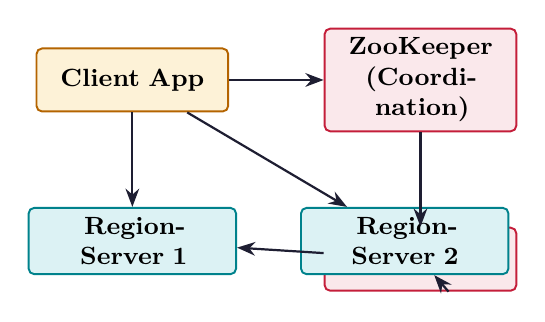
\begin{tikzpicture}[node distance=0.7cm and 0.8cm,
  mblock/.style={rectangle, draw=myred, fill=hdrred, text width=2.2cm, align=center, minimum height=0.8cm, font=\small\bfseries, rounded corners=2pt, line width=0.7pt},
  rblock/.style={rectangle, draw=myteal, fill=hdrteal, text width=2.4cm, align=center, minimum height=0.8cm, font=\small\bfseries, rounded corners=2pt, line width=0.7pt},
  cblock/.style={rectangle, draw=myamber, fill=hdramber, text width=2.2cm, align=center, minimum height=0.8cm, font=\small\bfseries, rounded corners=2pt, line width=0.7pt},
  bgbox/.style={draw=mgframe, fill=mygray, line width=0.8pt, rounded corners=4pt, inner sep=6pt}]

  % Nodes
  \node[cblock] (client) {Client App};
  \node[mblock, right=1.2cm of client] (zk) {ZooKeeper\\(Coordination)};
  \node[mblock, below=1.2cm of zk] (hm) {HMaster};

  \node[rblock, below=1.2cm of client] (rs1) {RegionServer 1};
  \node[rblock, right=0.8cm of rs1] (rs2) {RegionServer 2};

  % Connections
  \draw[arrow] (client) -- (zk);
  \draw[arrow] (zk) -- (hm);
  \draw[arrow] (client) -- (rs1);
  \draw[arrow] (client) -- (rs2);
  \draw[arrow] (hm) -- (rs1);
  \draw[arrow] (hm) -- (rs2);

\end{tikzpicture}
\end{tcolorbox}

% ===============================================================================
\section{IBM Big SQL}
% ===============================================================================

\begin{tcolorbox}[defbox, title={IBM Big SQL}]
  \textbf{IBM Big SQL} is an enterprise-grade, SQL-on-Hadoop engine that provides an ANSI-SQL compliant query compiler and Massively Parallel Processing (MPP) execution framework to query data stored across HDFS, Hive, and HBase directly.
\end{tcolorbox}

Big SQL utilizes a shared-nothing MPP architecture that executes SQL queries natively on Hadoop data blocks without the latency overhead of MapReduce translations, supporting complex joins and standard business intelligence integrations.

\newpage

% ═══════════════════════════════════════════════════════════════════════════════
% QUICK REVISION PAGE
% ═══════════════════════════════════════════════════════════════════════════════
\begin{center}
  {\large\bfseries\color{myred} Quick Revision --- Module 4}\\[3pt]
  {\small\color{mydark} Pig Latin, HiveQL, HBase NoSQL \& Big SQL $|$ OE-EC803B}
\end{center}
\noindent{\color{myred}\rule{\linewidth}{1.2pt}}
\vspace{8pt}

\begin{tcolorbox}[defbox, title={\textbf{One-Line Definitions}}]
\begin{itemize}[leftmargin=*, itemsep=3pt, topsep=0pt]
  \item \textbf{Pig Latin:} A high-level dataflow programming language used to describe data transformation pipelines.
  \item \textbf{HiveQL:} An SQL-like query language that is compiled into execution plans (like Tez or MapReduce).
  \item \textbf{Metastore:} The repository that stores structural metadata and schema information for Hive tables.
  \item \textbf{RegionServer:} An HBase slave node that serves read and write operations for a subset of row keys.
  \item \textbf{Big SQL:} An enterprise Massively Parallel Processing (MPP) SQL querying engine for Hadoop clusters.
\end{itemize}
\end{tcolorbox}

\vspace{6pt}

\begin{tcolorbox}[exambox, title={\textbf{Frequently Asked / Viva Questions}}]
\begin{enumerate}[leftmargin=*, topsep=0pt, label=\textbf{Q\arabic*.}, itemsep=5pt]
  \item \Q{Compare Apache Pig and Apache Hive.}
        Apache Pig uses a procedural dataflow scripting language (Pig Latin) suited for ETL pipelines and data engineers. Apache Hive uses a declarative SQL-like language (HiveQL) suited for data warehousing and business intelligence.
        
  \item \Q{What happens to the HDFS data when a Managed Table vs. an External Table is dropped in Hive?}
        Dropping a Managed Table deletes both the table metadata and the physical data files in HDFS. Dropping an External Table deletes only the Hive schema metadata, leaving the physical data files intact in HDFS.
        
  \item \Q{Explain the difference between Partitioning and Bucketing in Hive.}
        Partitioning organizes data into separate subdirectories based on column values (pruning queries). Bucketing splits data into a fixed number of files based on a hash of a column, which optimizes joins on high-cardinality columns.
        
  \item \Q{Detail the write path of a record in Apache HBase.}
        A client write is first appended to the Write-Ahead Log (WAL) on disk for durability, then written to the in-memory \textbf{MemStore} in RAM. Once the write is in MemStore, the client receives an ACK.
        
  \item \Q{When does HBase flush data, and what file format is generated?}
        When the in-memory MemStore reaches its capacity threshold (typically 128MB), HBase flushes its sorted key-value contents to HDFS, creating a new binary \textbf{HFile}.
        
  \item \Q{Why is HBase called a Column-Family NoSQL database?}
        HBase groups columns together into \textbf{Column Families} (defined during table creation). Internally, columns belonging to the same column family are stored in the same physical HFile, optimizing access for selective queries.
        
  \item \Q{What are the complex nested data types supported in Pig Latin?}
        \textbf{Tuple} (an ordered list of fields), \textbf{Bag} (an unordered collection of tuples), and \textbf{Map} (a set of key-value pairs).
        
  \item \Q{Explain the role of ZooKeeper in an HBase cluster.}
        ZooKeeper coordinates Region assignment, detects RegionServer failures, maintains the root table location, and prevents active-standby conflicts by coordinating HMaster elections.
        
  \item \Q{What are UDF, UDAF, and UDTF in Hive?}
        \begin{itemize}[leftmargin=*, noitemsep]
          \item \textbf{UDF:} User Defined Function (maps 1 row to 1 output).
          \item \textbf{UDAF:} User Defined Aggregate Function (maps multiple rows to 1 aggregated output).
          \item \textbf{UDTF:} User Defined Table Generating Function (maps 1 row to multiple output rows/tables).
        \end{itemize}
        
  \item \Q{Describe the execution flow of a Big SQL query.}
        Big SQL bypasses MapReduce. The Big SQL coordinator compiles SQL queries, optimizes execution plans, and uses an MPP engine to distribute query processing fragments directly to local nodes containing target HDFS blocks.
\end{enumerate}
\end{tcolorbox}

\vspace{6pt}

\begin{tcolorbox}[tikzbox, title={\textbf{Comparison Snapshot}}]
\textbf{Traditional RDBMS vs. NoSQL HBase:}\par\vspace{6pt}\noindent
{\renewcommand{\arraystretch}{1.4}%
\begin{tabularx}{\linewidth}{|B{3.2cm}|Y|Y|}
\hline
\textbf{Feature} & \textbf{Traditional RDBMS} & \textbf{NoSQL HBase} \\
\hline
Data Layout & Row-oriented (stores entire row together) & Column-family oriented (stores family columns together) \\
\hline
Schema Flexibility & Schema-on-write (rigid definitions) & Schema-less (columns can be added dynamically) \\
\hline
Transaction Support & Full ACID transactions across multiple tables & ACID transactions supported at Row-level only \\
\hline
Scaling Pattern & Vertical (bigger machines) & Horizontal (adding RegionServers in parallel) \\
\hline
Join Support & Rich declarative SQL joins & No native join support (requires MapReduce/Spark) \\
\hline
Null Value Storage & Consumes space for NULL definitions & Zero storage overhead for empty cells (sparse tables) \\
\hline
\end{tabularx}}
\end{tcolorbox}


% -- Module 5 -----------------------------------------------------------------
\modulestart{5}{R and Machine Learning in Big Data}

\section{R and Machine Learning in Big Data}
% ===============================================================================

Data analytics turns raw database bits into business value. R is a popular programming language for statistical computing and graphics. In Big Data architectures, statistical models are divided into supervised and unsupervised techniques:

\begin{tcolorbox}[defbox, title={Machine Learning Paradigms}]
  \begin{itemize}[leftmargin=*, itemsep=3pt]
    \item \textbf{Supervised Learning:} Training models using labeled datasets where the input features ($X$) are mapped to a known target variable ($Y$).
    \item \textbf{Unsupervised Learning:} Identifying hidden patterns, groups, or structures in unlabeled datasets where only input features ($X$) are provided.
  \end{itemize}
\end{tcolorbox}

\begin{tcolorbox}[tikzbox, title={Taxonomy of Machine Learning}]
\centering
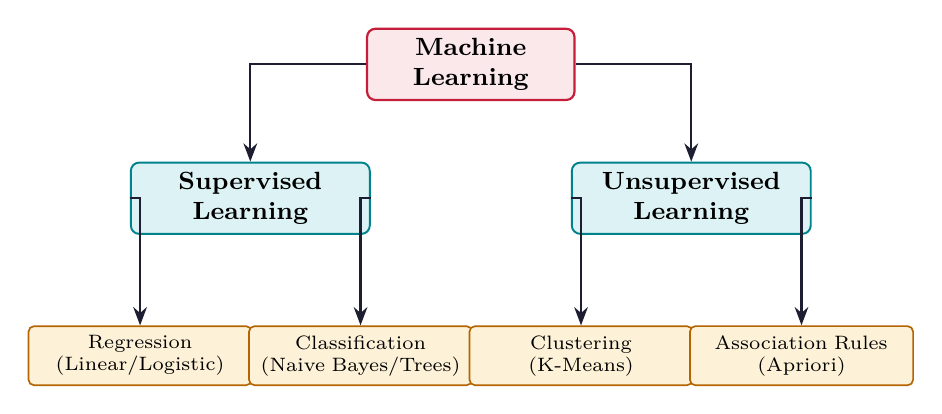
\begin{tikzpicture}[node distance=0.8cm and 0.4cm,
  root/.style={rectangle, draw=myred, fill=hdrred, text width=2.4cm, align=center, minimum height=0.8cm, font=\small\bfseries, rounded corners=3pt, line width=0.8pt},
  branch/.style={rectangle, draw=myteal, fill=hdrteal, text width=2.8cm, align=center, minimum height=0.75cm, font=\small\bfseries, rounded corners=3pt, line width=0.7pt},
  leaf/.style={rectangle, draw=myamber, fill=hdramber, text width=2.6cm, align=center, minimum height=0.75cm, font=\scriptsize, rounded corners=2pt, line width=0.6pt},
  carrow/.style={-Stealth, thick, color=mydark}]

  % Root
  \node[root] (ml) at (0,2.5) {Machine\\Learning};

  % Branches
  \node[branch] (sup) at (-2.8,0.8) {Supervised\\Learning};
  \node[branch] (unsup) at (2.8,0.8) {Unsupervised\\Learning};

  % Leaves
  \node[leaf] (reg) at (-4.2,-1.2) {Regression\\(Linear/Logistic)};
  \node[leaf] (clf) at (-1.4,-1.2) {Classification\\(Naive Bayes/Trees)};

  \node[leaf] (clust) at (1.4,-1.2) {Clustering\\(K-Means)};
  \node[leaf] (assoc) at (4.2,-1.2) {Association Rules\\(Apriori)};

  % Connections
  \draw[carrow] (ml) -| (sup);
  \draw[carrow] (ml) -| (unsup);
  \draw[carrow] (sup) -| (reg);
  \draw[carrow] (sup) -| (clf);
  \draw[carrow] (unsup) -| (clust);
  \draw[carrow] (unsup) -| (assoc);

\end{tikzpicture}
\end{tcolorbox}

% ===============================================================================
\section{Supervised Learning Algorithms}
% ===============================================================================

\subsection{Linear Regression}
Used to predict a continuous numeric output variable ($Y$) from one or more input features ($X$).

\begin{tcolorbox}[formulabox, title={Linear Regression Modeling}]
  The prediction hypothesis is modeled as:
  $$h_\theta(x) = \theta_0 + \theta_1 x_1 + \theta_2 x_2 + \dots + \theta_n x_n = \theta^T x$$
  The model parameters ($\theta_i$) are calculated by minimizing the \textbf{Mean Squared Error (MSE)} Cost Function:
  $$J(\theta) = \frac{1}{2m} \sum_{i=1}^{m} \left( h_\theta(x^{(i)}) - y^{(i)} \right)^2$$
  Parameters are updated iteratively using the \textbf{Gradient Descent} rule:
  $$\theta_j := \theta_j - \alpha \frac{\partial}{\partial \theta_j} J(\theta) = \theta_j - \alpha \frac{1}{m} \sum_{i=1}^{m} \left( h_\theta(x^{(i)}) - y^{(i)} \right) x_j^{(i)}$$
  *(where $\alpha$ is the learning rate parameter).*
\end{tcolorbox}

\subsection{Logistic Regression}
Despite its name, it is a classification algorithm used to predict binary categorical outcomes ($Y \in \{0, 1\}$).

\begin{tcolorbox}[formulabox, title={Sigmoid Function}]
  The prediction is modeled by feeding the linear hypothesis into the \textbf{Sigmoid (Logistic) Function} to output a probability between 0 and 1:
  $$h_\theta(x) = \sigma(\theta^T x) = \frac{1}{1 + e^{-\theta^T x}}$$
  \begin{itemize}[leftmargin=*, noitemsep]
    \item If $h_\theta(x) \geq 0.5 \implies \text{Predict } 1$
    \item If $h_\theta(x) < 0.5 \implies \text{Predict } 0$
  \end{itemize}
\end{tcolorbox}

\subsection{Decision Trees}
A non-parametric model that builds a tree hierarchy by splitting datasets based on features that maximize purity:
\begin{itemize}[leftmargin=*, itemsep=3pt]
  \item \textbf{Entropy:} Measures the impurity or randomness of a dataset:
    $$H(S) = -\sum_{i=1}^{c} p_i \log_2 p_i$$
  \item \textbf{Information Gain:} Measures the reduction in entropy after splitting on a feature $A$:
    $$IG(S, A) = H(S) - \sum_{v \in Values(A)} \frac{|S_v|}{|S|} H(S_v)$$
\end{itemize}

\subsection{Naive Bayes Classification}
A probabilistic classification algorithm based on Bayes' Theorem:

\begin{tcolorbox}[formulabox, title={Bayes' Theorem and Naive Assumption}]
  $$P(C_k \mid x) = \frac{P(x \mid C_k) P(C_k)}{P(x)}$$
  \textbf{Naive conditional independence assumption:} Assumes that the presence of a particular feature in a class is completely independent of the presence of any other feature:
  $$P(x_1, x_2, \dots, x_n \mid C_k) = \prod_{i=1}^{n} P(x_i \mid C_k)$$
  Combining these yields the Naive Bayes classification rule:
  $$\hat{y} = \arg\max_{k} P(C_k) \prod_{i=1}^{n} P(x_i \mid C_k)$$
\end{tcolorbox}

% ===============================================================================
\section{Unsupervised Learning Algorithms}
% ===============================================================================

\subsection{K-Means Clustering}
An iterative clustering algorithm that partitions $m$ data points into $K$ distinct, non-overlapping groups (clusters):
\begin{enumerate}[leftmargin=*, itemsep=3pt]
  \item \textbf{Initialize:} Randomly choose $K$ centroids ($\mu_1, \mu_2, \dots, \mu_K$).
  \item \textbf{Assign:} Group each data point $x^{(i)}$ to its closest centroid:
    $$c^{(i)} := \arg\min_j ||x^{(i)} - \mu_j||^2$$
  \item \textbf{Update:} Recompute the centroid values as the mean of all data points assigned to that cluster:
    $$\mu_j := \frac{\sum_{i=1}^{m} \mathbb{I}(c^{(i)} = j) x^{(i)}}{\sum_{i=1}^{m} \mathbb{I}(c^{(i)} = j)}$$
  \item \textbf{Repeat:} Repeat steps 2 and 3 until centroids stop changing.
\end{enumerate}

\subsection{Association Rule Mining: Apriori Algorithm}
Used to identify relationships between variables in large transaction databases (e.g., market basket analysis).

\begin{tcolorbox}[formulabox, title={Association Rule Metrics}]
  An association rule is written as $X \rightarrow Y$ (e.g., $\{Bread\} \rightarrow \{Butter\}$).
  \begin{itemize}[leftmargin=*, itemsep=3pt]
    \item \textbf{Support:} The fraction of total transactions containing both itemsets:
      $$Support(X \rightarrow Y) = \frac{\text{Count}(X \cup Y)}{N}$$
    \item \textbf{Confidence:} How often items in $Y$ appear in transactions containing $X$:
      $$Confidence(X \rightarrow Y) = \frac{Support(X \cup Y)}{Support(X)}$$
    \item \textbf{Lift:} The ratio of the rule's confidence to its expected confidence under independence:
      $$Lift(X \rightarrow Y) = \frac{Confidence(X \rightarrow Y)}{Support(Y)}$$
      *(If $Lift > 1$, items are highly dependent; if $Lift < 1$, they are substitutes).*
  \end{itemize}
\end{tcolorbox}

The \textbf{Apriori Algorithm} uses the downward closure property: \textit{all subsets of a frequent itemset must also be frequent}. If an itemset is infrequent, all its supersets are pruned immediately.

% ===============================================================================
\section{Collaborative Filtering}
% ===============================================================================

\begin{tcolorbox}[defbox, title={Collaborative Filtering}]
  \textbf{Collaborative Filtering} is a recommendation system technique that filters information or patterns using the preferences or historical behaviors of multiple users, based on the assumption that users who agreed in the past will agree in the future.
\end{tcolorbox}

Two main collaborative filtering patterns are:
\begin{enumerate}[leftmargin=*, itemsep=3pt]
  \item \textbf{User-Based Collaborative Filtering:} Identifies users similar to the active user (based on rating history) and recommends items that those similar users liked.
  \item \textbf{Item-Based Collaborative Filtering:} Calculates similarities between items based on user ratings. Recommends items similar to those the active user rated highly in the past.
\end{enumerate}

\begin{tcolorbox}[formulabox, title={Cosine Similarity Metric}]
  The similarity between two user rating vectors (or item rating vectors) $A$ and $B$ is measured using \textbf{Cosine Similarity}:
  $$\text{Similarity}(A, B) = \cos(\theta) = \frac{A \cdot B}{||A|| \, ||B||} = \frac{\sum_{i} A_i B_i}{\sqrt{\sum_{i} A_i^2} \sqrt{\sum_{i} B_i^2}}$$
\end{tcolorbox}

% ===============================================================================
\section{Big Data Analytics with BigR}
% ===============================================================================

Standard R loads all data structures entirely into the local machine's RAM. If a dataset is 1TB, native R will crash with out-of-memory errors.

\begin{tcolorbox}[defbox, title={BigR}]
  \textbf{BigR} is an enterprise R package that provides a client-side interface connecting R sessions directly to IBM InfoSphere BigInsights or Apache Spark clusters, allowing users to execute statistics and machine learning on distributed datasets in parallel.
\end{tcolorbox}

BigR uses \textbf{deferred execution} to translate R commands into MapReduce or SQL operations that run directly on HDFS data blocks, returning only the final, aggregated results back to the user's local R terminal.

\newpage

% ═══════════════════════════════════════════════════════════════════════════════
% QUICK REVISION PAGE
% ═══════════════════════════════════════════════════════════════════════════════
\begin{center}
  {\large\bfseries\color{myred} Quick Revision --- Module 5}\\[3pt]
  {\small\color{mydark} Machine Learning, Association Rules \& BigR $|$ OE-EC803B}
\end{center}
\noindent{\color{myred}\rule{\linewidth}{1.2pt}}
\vspace{8pt}

\begin{tcolorbox}[defbox, title={\textbf{One-Line Definitions}}]
\begin{itemize}[leftmargin=*, itemsep=3pt, topsep=0pt]
  \item \textbf{Supervised Learning:} Training models using input-output pairs to predict targets for unseen data.
  \item \textbf{Unsupervised Learning:} Finding patterns in data without using target labels.
  \item \textbf{Entropy:} A thermodynamic-inspired metric measuring the impurity of a dataset split.
  \item \textbf{Collaborative Filtering:} Making recommendations by comparing user rating histories.
  \item \textbf{BigR:} An R package that runs parallel analytical calculations on distributed Hadoop clusters.
\end{itemize}
\end{tcolorbox}

\vspace{6pt}

\begin{tcolorbox}[exambox, title={\textbf{Frequently Asked / Viva Questions}}]
\begin{enumerate}[leftmargin=*, topsep=0pt, label=\textbf{Q\arabic*.}, itemsep=5pt]
  \item \Q{What is the difference between Linear and Logistic Regression?}
        Linear regression predicts continuous numeric variables (e.g., salary, price) by fitting a straight line. Logistic regression classifies binary categorical variables (e.g., spam/not-spam) by passing a linear hypothesis through the sigmoid function to output probabilities.
        
  \item \Q{Detail the mathematical steps of Gradient Descent.}
        It starts with random parameter values ($\theta$). In each iteration, it computes the gradient (partial derivative) of the Cost Function $J(\theta)$ with respect to each parameter, and updates the parameters in the direction of the steepest descent: $\theta_j := \theta_j - \alpha \frac{\partial}{\partial \theta_j} J(\theta)$.
        
  \item \Q{Explain the role of Entropy in Decision Tree splits.}
        Entropy measures the impurity of a node: $H(S) = -\sum p_i \log_2 p_i$. The decision tree algorithm calculates the entropy of the current node, splits the data using a feature, and computes the entropy of the child nodes. It selects the feature that maximizes the reduction in entropy (Information Gain).
        
  \item \Q{Why is Naive Bayes called ``Naive''?}
        Because it assumes that all input features are conditionally independent of each other given the class label. In reality, features are often correlated (e.g., height and weight). Despite this assumption, it works well in practice for text classification.
        
  \item \Q{How does the K-Means clustering algorithm converge?}
        It converges when the assignments of data points to clusters stop changing, or when the positions of the cluster centroids remain constant across iterations, minimizing the total within-cluster sum of squared errors.
        
  \item \Q{What is the difference between Support and Confidence in the Apriori algorithm?}
        Support is the percentage of all transactions that contain the itemset ($Support(X \cup Y)$). Confidence is the conditional probability that a transaction contains $Y$ given that it contains $X$ ($Support(X \cup Y) / Support(X)$).
        
  \item \Q{Why does the Apriori algorithm prune infrequent itemsets?}
        Because of the Apriori property: *if an itemset is frequent, all its subsets must be frequent*. Conversely, if an itemset is infrequent, all its supersets must also be infrequent, allowing them to be pruned immediately.
        
  \item \Q{Compare User-Based and Item-Based Collaborative Filtering.}
        User-Based filtering calculates similarities between users to recommend items. It scales poorly because user preferences change frequently. Item-Based filtering calculates similarities between items. Since item attributes are static, these similarity matrices can be computed offline, making it more scalable.
        
  \item \Q{How is Cosine Similarity used in recommendation engines?}
        It measures the similarity between two rating vectors by calculating the cosine of the angle between them: $\frac{A \cdot B}{||A|| \, ||B||}$. A value of 1 indicates identical rating patterns, while 0 indicates orthogonal (dissimilar) patterns.
        
  \item \Q{Why is native R unsuited for Big Data, and how does BigR resolve this?}
        Native R loads all data structures directly into memory, which crashes on large datasets. BigR acts as an API gateway, translating R commands into SQL or MapReduce operations that run directly on HDFS, avoiding memory bottlenecks.
\end{enumerate}
\end{tcolorbox}

\vspace{6pt}

\begin{tcolorbox}[tikzbox, title={\textbf{Comparison Snapshot}}]
\textbf{Supervised vs. Unsupervised Machine Learning:}\par\vspace{6pt}\noindent
{\renewcommand{\arraystretch}{1.4}%
\begin{tabularx}{\linewidth}{|B{3.2cm}|Y|Y|}
\hline
\textbf{Feature} & \textbf{Supervised Learning} & \textbf{Unsupervised Learning} \\
\hline
Input Data & Labeled training datasets (features + target labels) & Unlabeled datasets (features only) \\
\hline
Primary Goal & Predict target outputs ($Y$) for new, unseen inputs ($X$) & Uncover hidden structures, patterns, or groupings \\
\hline
Evaluation & Metrics: Accuracy, Precision, Recall, MSE, $R^2$ & Metrics: Silhouette score, Inertia, Lift \\
\hline
Algorithms & Linear/Logistic Regression, Naive Bayes, Decision Trees & K-Means Clustering, Apriori, Principal Component Analysis \\
\hline
Complexity & High supervision required (data labeling is expensive) & Low supervision; patterns are discovered automatically \\
\hline
\end{tabularx}}
\end{tcolorbox}


\end{document}
